\documentclass[12pt,a4paper]{article}

% Paragraphs: single line spacing, light separation between paragraphs
\setlength{\parindent}{15pt}
\setlength{\parskip}{0.4\baselineskip}

% Line spacing per norms SAE Geneve: 1.5 for body text (footnotes stay single-spaced by default with setspace)
\usepackage{setspace}
\onehalfspacing

% Language setting
\usepackage[T1]{fontenc}
\usepackage[english]{babel}

% Use Times-like font (recommended for academic documents)
\usepackage{newtxtext,newtxmath}

% For figures and tables
\usepackage{graphicx}
\graphicspath{{img/}}
\usepackage{microtype}
\usepackage{array}

% hyperref must be loaded before glossaries for \gls links to work correctly
\usepackage[colorlinks=true, allcolors=blue]{hyperref}

% Glossary
\usepackage[toc, acronym]{glossaries}
\setacronymstyle{long-short-desc}
\makeglossaries
% =========================================
% === Italicised call for anglicisms ===
% Wraps \gls / \glspl in \textit for entries
% that are English common-noun anglicisms
% (not proper nouns/brand names, not French
% translations, not acronyms).
% =========================================
\newcommand{\glsit}[1]{\textit{\gls{#1}}}
\newcommand{\glsplit}[1]{\textit{\glspl{#1}}}

% ==========================
% ======== Acronyms ========
% ==========================

\newacronym[description={}]{vn}{VN}{Visual Novel}
%\newacronym[plural=vn,firstplural={Visual Novels} (VN)]{vn}{VN}{Visual Novel}
%\newacronym[description={}]{ia}{I.A.}{Intelligence Artificielle}
\newacronym[description={}]{json}{JSON}{JavaScript Object Notation}
\newacronym[description={}]{yaml}{YAML}{YAML Ain't Markup Language}
\newacronym[description={}]{toml}{TOML}{Tom's Obvious, Minimal Language}
\newacronym[description={}]{html}{HTML}{HyperText Markup Language}
\newacronym[description={}]{dom}{DOM}{Document Object Model (\textit{Modèle Objet de Document})}
\newacronym[description={}]{css}{CSS}{Cascading Style Sheets (\textit{Feuilles de Style en Cascade})}



% ============================
% ======== Glossaries ========
% ============================

\newglossaryentry{opensource}{
    name={open source},
    description={Modèle de développement dans lequel le code source est public et peut être consulté, modifié et redistribué par tous, selon les conditions de sa licence}
}

\newglossaryentry{js}{
    name={JavaScript},
    description={Langage de programmation exécuté nativement dans les
navigateurs web, utilisé pour rendre les pages interactives et dynamiques.
Il constitue la base technique de ce projet: \gls{reactjs}, la \gls{librairie}
utilisée pour le moteur, est écrite en JavaScript, et le format \acrshort{json} est
directement interprétable par ce langage sans dépendance externe}
}

\newglossaryentry{ts}{
    name={TypeScript},
    description={Surcouche typée de \gls{js}, développée par Microsoft, qui ajoute un système de types statiques au langage. Les types permettent de détecter à la compilation des erreurs qui ne seraient pas visibles à l'exécution en \gls{js} pur. TypeScript est compilé vers \gls{js} standard avant d'être exécuté dans le navigateur \parencite{noauthor_starting_nodate}}
}

\newglossaryentry{reactjs}{
    name={React.js},
    description={Bibliothèque \gls{js} développée par Meta, utilisée pour construire des interfaces web interactives sous forme de composants réutilisables. Ce projet repose sur React.js pour le rendu du moteur de \acrlong{vn} dans le navigateur}
}

\newglossaryentry{frontend}{
    name={frontend},
    description={Partie d'une application web exécutée directement dans le navigateur de l'utilisateur, responsable de l'affichage et des interactions. S'oppose au \glsit{backend}, qui désigne la partie serveur}
}

\newglossaryentry{syntaxe}{
    name={syntaxe},
    description={Ensemble des règles formelles qu'un fichier ou un script doit respecter pour être correctement interprété par un programme. Dans ce projet, ce terme désigne notamment les règles structurelles du format \acrshort{json} utilisé comme source de contenu du moteur}
}

\newglossaryentry{parseur}{
    name={parseur},
    description={Programme ou composant logiciel chargé de lire un fichier texte et d'en interpréter la structure selon des règles définies. Dans ce projet, le parseur analyse le fichier \acrshort{json} du scénario et vérifie qu'il est conforme au \gls{schema} attendu avant de le transmettre au moteur}
}

\newglossaryentry{schema}{
    name={schéma},
    description={Au sens informatique, description formelle de la structure attendue d'un fichier de données: quels champs sont obligatoires, quels types de valeurs sont acceptés, et comment les éléments sont organisés. Dans ce projet, le schéma \acrshort{json} définit la structure que doit respecter tout fichier de scénario pour être reconnu et exécuté par le moteur}
}

\newglossaryentry{librairie}{
    name={librairie},
    description={Dans le domaine du développement logiciel, ensemble de composants ou de fonctions réutilisables qu'un développeur peut intégrer dans son propre projet. À ne pas confondre avec son sens courant: il ne s'agit pas d'un lieu physique, mais d'un module logiciel distribuable}
}

\newglossaryentry{nocode}{
    name={no-code/low-code},
    description={Approches de développement logiciel visant à réduire ou 
    supprimer la nécessité d'écrire du code. Les outils no-code reposent 
    entièrement sur des interfaces visuelles, tandis que les outils low-code 
    permettent d'y adjoindre du code pour des besoins spécifiques. Ces 
    approches visent à rendre la création d'applications accessible à des 
    utilisateurs sans formation technique}
}

\newglossaryentry{webassembly}{
    name={WebAssembly},
    description={Format d'instructions binaires permettant d'exécuter dans un navigateur web du code compilé depuis d'autres langages que \gls{js}, avec des performances proches du natif}
}

\newglossaryentry{backend}{
    name={backend},
    description={Partie serveur d'une application web, invisible à l'utilisateur final, qui gère la logique métier, le stockage des données et les traitements nécessitant un environnement sécurisé}
}

\newglossaryentry{npm}{
    name={npm},
    description={Gestionnaire de paquets pour \gls{js}, installé avec Node.js. Il permet d'installer, de mettre à jour et de publier des \glspl{librairie} réutilisables (appelées \glsplit{package}) dans un projet \gls{js} ou \gls{ts}. La commande \texttt{npm install} télécharge les dépendances d'un projet, et \texttt{npm run build} exécute un script de compilation défini dans le fichier \texttt{package.json}}
}

\newglossaryentry{package}{
    name={package},
    description={Dans le domaine du développement \gls{js}, module logiciel distribué via \gls{npm}, installable dans un projet par une commande. Un package peut être une \gls{librairie} (comme \gls{reactjs} ou \gls{zod}), un outil de \glsit{build} (comme \gls{vite}), ou tout autre ensemble de fonctionnalités réutilisables. À ne pas confondre avec son sens courant de colis ou paquet physique}
}

\newglossaryentry{webworker}{
    name={Web Worker},
    description={Mécanisme natif des navigateurs web permettant d'exécuter du code \gls{js} dans un fil d'exécution secondaire, séparé du fil principal gérant l'interface utilisateur. Cela permet de déléguer des traitements coûteux en calcul sans bloquer l'affichage ni les interactions de l'utilisateur. Les Web Workers communiquent avec le fil principal par échange de messages, sans accès direct au \acrshort{dom} \parencite{noauthor_utilisation_2025}}
}

\newglossaryentry{plugin}{
    name={plugin},
    description={Module logiciel externe venant s'intégrer à un outil existant pour en étendre les fonctionnalités sans modifier son code source}
}

\newglossaryentry{override}{
    name={surcharge},
    description={(\textit{override}) En développement logiciel, mécanisme permettant de remplacer localement une valeur ou un comportement défini globalement, sans modifier la définition globale}
}

\newglossaryentry{tokenisation}{
    name={tokenisation},
    description={Processus de découpage d'une chaîne de texte en unités élémentaires appelées \textit{tokens}}
}

\newglossaryentry{markdown}{
    name={Markdown},
    description={Langage de balisage léger créé par John Gruber en 2004, conçu pour être lisible sous forme brute tout en pouvant être converti en \acrshort{html} \parencite{noauthor_daring_nodate}}
}

\newglossaryentry{framework}{
    name={framework},
    description={Cadre de développement logiciel fournissant une structure imposée et des outils intégrés pour la construction d'application. À distinguer d'une \gls{librairie} : un framework dicte l'architecture du projet, tandis qu'une \gls{librairie} s'intègre dans une architecture existante au choix du développeur}
}

\newglossaryentry{rendu}{
    name={rendu},
    description={(\textit{render}) En développement d'interfaces web, processus par lequel le navigateur calcule et met à jour l'affichage d'un composant en réponse à un changement d'état ou de données. Dans le contexte de \gls{reactjs}, un rendu désigne spécifiquement l'exécution de la fonction d'un composant et le recalcul de son arbre \acrshort{html} virtuel. Un rendu inutile survient lorsqu'un composant est recalculé sans que ses données aient changé}
}

\newglossaryentry{zod}{
    name={Zod},
    description={\Gls{librairie} de validation de \gls{schema} et d'inférence de types pour \gls{ts}, développé par Colin McDonnell \parencite{noauthor_zod_nodate}. Elle permet de définir la structure attendue d'un objet et de valider des données à l'exécution, en produisant des messages d'erreur précis en cas de non-conformité}
}

\newglossaryentry{hook}{
    name={hook},
    description={Dans \gls{reactjs}, fonction spéciale dont le nom commence par \texttt{use}, permettant d'accéder à des fonctionnalités du cycle de vie et de l'état d'un composant depuis une fonction \gls{js} ordinaire \parencite{noauthor_reference_nodate}}
}

\newglossaryentry{git}{
    name={Git},
    description={Système de gestion de versions distribué créé par Linus Torvalds en 2005 \parencite{noauthor_git_nodate}, permettant de suivre l'historique des modifications d'un projet, de travailler sur des branches parallèles et de collaborer à plusieurs sur un même code source}
}

\newglossaryentry{moscow}{
    name={MoSCoW},
    description={Méthode de priorisation des exigences issue de la gestion de projet agile. L'acronyme désigne quatre niveaux de priorité: \textit{Must have} (indispensable), \textit{Should have} (important mais non bloquant), \textit{Could have} (souhaitable si le temps le permet) et \textit{Won't have} (hors périmètre pour cette itération) \parencite{clegg_case_1994}}
}

\newglossaryentry{pdca}{
    name={PDCA},
    description={Cycle d'amélioration continue en quatre phases: \textit{Plan} (planification), \textit{Do} (mise en \oe{}uvre), \textit{Check} (évaluation) et \textit{Act} (ajustement). Formalisé par W. Edwards Deming \parencite{deming_out_1986}}
}

\newglossaryentry{vite}{
    name={Vite},
    description={Outil de \glsit{build} et serveur de développement \glsit{frontend} développé par Evan You, conçu pour offrir un rechargement à chaud rapide et une compilation optimisée pour les projets \gls{js} modernes \parencite{noauthor_vite_nodate}}
}

\newglossaryentry{poc}{
    name={proof of concept},
    description={Démonstration ou prototype fonctionnel visant à vérifier la faisabilité technique d'une idée ou d'une approche, sans nécessairement couvrir l'ensemble des cas d'usage ni atteindre un niveau de finition production}
}

\newglossaryentry{snaphtml}{
    name={snapshot HTML},
    description={Dans le contexte du composant \texttt{Typewriter}, désigne une chaîne de caractères représentant l'état complet du \gls{rendu} \acrshort{html} à un instant donné de l'animation machine à écrire. Chaque snapshot correspond à un nombre précis de caractères visibles affichés, avec les balises \acrshort{html} ouvertes et fermées correctement, permettant un affichage en O(1) par tick d'animation (Auteur 2026)}
}

\newglossaryentry{sprite}{
    name={sprite},
    description={Image ou illustration représentant un personnage ou un élément graphique, affichée par-dessus le décor d'une scène et pouvant être positionnée ou animée indépendamment de celui-ci. Terme issu du développement de jeux vidéo en deux dimensions}
}

\newglossaryentry{memoisation}{
    name={mémoïsation},
    description={Technique d'optimisation consistant à mettre en cache le résultat d'un calcul ou d'un appel de fonction coûteux, afin de le réutiliser lors d'appels ultérieurs avec les mêmes paramètres plutôt que de le recalculer. À ne pas confondre avec la mémorisation au sens cognitif: il s'agit ici d'un terme technique adapté de l'anglais \textit{memoization}, désignant ce mécanisme de cache}
}

\newglossaryentry{runtime}{
    name={runtime},
    description={Environnement d'exécution d'un programme, par opposition à sa compilation. Désigne aussi, par extension, le composant logiciel chargé d'interpréter et d'exécuter un contenu à ce moment-là, par exemple le moteur qui interprète un fichier de scénario dans le navigateur}
}

\newglossaryentry{placeholder}{
    name={placeholder},
    description={Texte ou valeur temporaire affiché dans un champ de saisie vide, servant d'indication à l'utilisateur sur le contenu attendu, et disparaissant dès que celui-ci commence à saisir une valeur}
}

\newglossaryentry{build}{
    name={build},
    description={Processus de compilation et d'assemblage du code source d'un projet en fichiers optimisés, prêts à être déployés. Dans ce projet, cette étape est exécutée par la commande \texttt{npm run build}}
}

\newglossaryentry{negativetesting}{
    name={negative testing},
    description={(\textit{unhappy path testing}) Approche de test visant à vérifier le comportement d'un programme face à des entrées inattendues, invalides ou erronées, par opposition au \textit{positive testing}, qui couvre le comportement attendu en conditions normales. Hora définit les tests négatifs comme ceux qui vérifient «l'exécution anormale, comme les cas exceptionnels» \parencite{hora_test_2024}}
}

\newglossaryentry{reactprofiler}{
    name={React DevTools Profiler},
    description={Extension de navigateur développée par Meta Open Source permettant d'enregistrer et d'analyser les performances de rendu d'une application \gls{reactjs}, notamment la durée et la fréquence des cycles de \gls{rendu} par composant \parencite{noauthor_react_nodate}}
}

% Set page size and margins
% Replace `letterpaper' with `a4paper' for UK/EU standard size
\usepackage[a4paper,top=2.5cm,bottom=2.5cm,left=2.5cm,right=2.5cm,marginparwidth=1.75cm]{geometry}

% Useful packages
\usepackage{amsmath}
% (graphicx already loaded)
\usepackage{booktabs}
\usepackage[]{mdframed}
\usepackage{datetime2}
\usepackage{titlesec}
\usepackage{subcaption}
\usepackage{minted}
\usepackage{tablefootnote}
\usepackage{pdfpages}


\usepackage{tikz}
\usetikzlibrary{arrows.meta, positioning, fit, backgrounds}
\usepackage{xcolor}


% ----------------------------------------------------------

% Couleurs
\definecolor{clrInput}   {HTML}{D6EAF8}
\definecolor{clrProcess} {HTML}{FEF9E7}
\definecolor{clrToken}   {HTML}{D5F5E3}
\definecolor{clrOutput}  {HTML}{FADBD8}
\definecolor{clrBorder}  {HTML}{2C3E50}
\definecolor{clrArrow}   {HTML}{1A252F}
\definecolor{clrNote}    {HTML}{7F8C8D}

\definecolor{clrAuteur} {HTML}{D6EAF8}
\definecolor{clrBuild}  {HTML}{FEF9E7}
\definecolor{clrCloud}  {HTML}{D5F5E3}
\definecolor{clrPlayer} {HTML}{FADBD8}
\definecolor{clrAlt}    {HTML}{EBE2F5}
\definecolor{clrBorder} {HTML}{2C3E50}
\definecolor{clrArrow}  {HTML}{1A252F}
\definecolor{clrNote}   {HTML}{7F8C8D}

% ----------------------------------------------------------


\usepackage{pgfplots}
\pgfplotsset{compat=1.18}


\usepackage[style=ext-authoryear, backend=biber]{biblatex}
\addbibresource{references.bib} % note the .bib is required

% Page numbering position: bottom right instead of default bottom center
\usepackage{fancyhdr}
\pagestyle{fancy}
\fancyhf{}
\fancyfoot[R]{\thepage}
\renewcommand{\headrulewidth}{0pt}
\fancypagestyle{plain}{%
  \fancyhf{}
  \fancyfoot[R]{\thepage}
  \renewcommand{\headrulewidth}{0pt}
}


% ----------------------------------------------------------

\newcommand{\ns}{NamelessStory}
\newcommand{\nsit}{\textit{\ns}}
\newcommand{\nsits}{\nsit\space}
\newcommand{\nsrepo}{\url{https://github.com/NamelessProj/NamelessStory}}

% ----------------------------------------------------------


% ----------------------------------------------------------

\renewcommand{\listingscaption}{Code excerpt}
\renewcommand{\listoflistingscaption}{List of code excerpts}

% ----------------------------------------------------------


% ----------------------------------------------------------

\titleclass{\subsubsubsection}{straight}[\subsection]

\newcounter{subsubsubsection}[subsubsection]
\renewcommand\thesubsubsubsection{\thesubsubsection.\arabic{subsubsubsection}}

\titleformat{\subsubsubsection}
  {\normalfont\normalsize\bfseries}{\thesubsubsubsection}{1em}{}
\titlespacing*{\subsubsubsection}
{0pt}{3.25ex plus 1ex minus .2ex}{1.5ex plus .2ex}
\makeatletter
\def\toclevel@subsubsubsection{4}
\def\l@subsubsubsection{\@dottedtocline{4}{7em}{4em}}
\makeatother
\setcounter{secnumdepth}{4}
\setcounter{tocdepth}{4}

% ----------------------------------------------------------


\DTMsetdatestyle{ddmmyyyy}

\title{Bachelor Thesis - Da Silva Pinto Kevin}
\author{Da Silva Pinto Kevin}

\begin{document}



% ----------------------------------------------------------
% Page de garde

\pagenumbering{gobble}

\includepdf[pages=1-2]{Page_Garde_MemoireSAE.pdf}
\clearpage
\pagenumbering{roman}

% ----------------------------------------------------------



\addcontentsline{toc}{section}{Abstract}
\section*{Abstract}

This thesis presents the design and implementation of \nsit, a web \acrlong{vn} engine built on a declarative \acrshort{json} file. The project stems from a personal observation: existing \acrlong{vn} engines often offer rich features, but impose compilation steps, external dependencies, or deployment pipelines that complicate the task for a non-developer author who simply wants to tell an interactive story. The goal of the project was therefore to test whether a more direct architecture, driven solely by a declarative script interpreted in the browser, could allow this type of author to create and publish interactive content without any installation or compilation on the user's side.

To achieve this, I structured the development around a \glsit{pdca} cycle across three iterations: setting up the engine's foundations, optimising \gls{rendu}, and strengthening robustness. The work resulted in a \glsit{runtime} built in \gls{ts}/\gls{reactjs}, declarative data validation via the \gls{zod} \gls{librairie}, and several mechanisms dedicated to narrative navigation, progressive text display, and the handling of choices and branching.

The results show that it is technically possible to describe an interactive narrative with a simple declarative format and run it directly in a browser, without a \glsit{backend}. The optimisation iteration reduced the number of \glspl{rendu} required by 28.5\%, and validation via \gls{zod} reliably detects \acrshort{json} \gls{syntaxe} errors as well as corrupted save files. However, the \acrshort{json} format remains demanding for a non-technical author, which confirms that an engine of this kind should ideally be complemented by a guided editing tool to be truly accessible to non-developer authors.

\medskip
\noindent\textbf{Keywords:} \textit{Visual Novel}, declarative script, JSON, no-code/low-code, interactive narration.

\clearpage

\addcontentsline{toc}{section}{Preface}
\section*{Preface}

I discovered \glslink{vn}{Visual Novels} almost by chance, coming across \textit{Higurashi When They Cry Hou - Ch.1 Onikakushi} while browsing Steam. What struck me first was not the genre's technical complexity, but on the contrary the way it manages to create real narrative tension with very simple means: text, still images, and music.

As I kept exploring this type of work, my interest grew stronger. The more I saw what a \acrlong{vn} could tell, the more concrete the urge to create my own story became. At the same time, I quickly ran into the limits of existing tools. RenPy requires learning a dedicated scripting language. Twine demands a learning curve that remains too heavy for someone who mainly wants to write rather than configure an environment.

It is this frustration that gave rise to \nsit. At first, I simply wanted to build a personal \gls{reactjs} \gls{librairie} to run my own \acrlong{vn}. The project then took a different direction: it became an \glsit{opensource} engine, accessible from a browser, designed so that someone with basic \acrshort{json} skills could create and publish a story without any particular installation.

This preface therefore summarises the project's starting point: a personal idea, born from a very concrete use of the genre, which gradually evolved into a tool meant to be shared.

\clearpage

\addcontentsline{toc}{section}{Acknowledgements}
\section*{Acknowledgements}

I would first like to thank Jenna Luthi and Julien Ramirez for their guidance throughout this work. Their feedback helped me keep a clear direction, better frame certain decisions, and avoid scattering my efforts across secondary directions.

I would also like to thank Serge, who took the time to discuss technical aspects with me, advise me on the writing, and suggest useful directions for moving the work forward.

I would also like to thank the people who supported me while working on this thesis, in particular my family and those close to me. Their presence mattered just as much during moments of doubt as during periods when the project was moving forward quickly.

\clearpage

% Table of contents ====
\begin{singlespace}
\addcontentsline{toc}{section}{Table of Contents}
\tableofcontents
\end{singlespace}
\clearpage
% =======================

% Lists =================
\begin{singlespace}
\addcontentsline{toc}{section}{List of Figures}
\listoffigures

\addcontentsline{toc}{section}{List of Tables}
\listoftables

\clearpage

\addcontentsline{toc}{section}{List of Code Excerpts}
\listoflistings
\end{singlespace}
% =======================

% Glossary ===============
\printglossaries
\clearpage
% =======================

% Note liminaire =========
\addcontentsline{toc}{section}{Note on Terminology}
\section*{Note on Terminology}

This thesis makes use of numerous technical terms specific to web development. Recurring terms, appearing across several chapters, are defined once in the glossary above: each occurrence links back to it, and informal or slang technical terms are typeset in italics there. Terms that appear only occasionally, and do not warrant a glossary entry, are explained directly in a footnote at their first occurrence.

\clearpage
% =======================

\pagenumbering{arabic}

% ==========================
% ======== CHAPTERS ========
% ==========================



\section{Introduction}

Ce chapitre pose le cadre du projet et explique pourquoi j’ai choisi de travailler sur un moteur de \gls{vn} web piloté par un script déclaratif. Il présente le contexte, la problématique, les objectifs et la méthode retenue, afin de préciser ce que ce mémoire cherche réellement à démontrer.

\subsection{Contexte}
Le genre du \gls{vn} combine narration, images et sons pour proposer des expériences interactives centrées sur le récit. Ce qui m’a intéressé dans ce format, c’est qu’il met le texte au centre, tout en laissant de la place à la mise en scène et à l’interactivité. En pratique, les moteurs existants offrent souvent des fonctionnalités très complètes, mais ils imposent aussi des étapes de compilation, des dépendances externes ou des chaînes de déploiement qui compliquent la tâche d’un auteur non-développeur. J’ai donc cherché une alternative plus directe: un moteur de \gls{vn} destiné au web, capable d’interpréter un fichier déclaratif sans installation ni compilation côté auteur.

\subsection{Problématique}
La question centrale est la suivante : dans quelle mesure une architecture de moteur de \acrlong{vn} web, basée sur un format de script déclaratif, permet-elle à des auteurs non-développeurs de créer et de déployer du contenu interactif ? Derrière cette question, il y a un point très concret: est-ce qu’un auteur peut se concentrer sur son histoire, tout en utilisant un format suffisamment simple pour rester lisible, exploitable et publiable directement dans un navigateur ?

\clearpage

\subsection{Objectifs}
Les objectifs retenus pour ce projet sont expliqués dans le tableau \ref{tab:objectifs_moscow_intro} en utilisant le système de priorisation \glsit{moscow}.

\begin{table}[H]
    \centering
    \caption{Objectifs du projet (priorisation MoSCoW)}
    \renewcommand{\arraystretch}{1.4}
    \begin{tabular}{p{1.8cm} p{11.5cm}}
        \hline
        \textbf{Priorité} & \textbf{Objectif} \\
        \hline
        Must & Concevoir et implémenter un moteur de \gls{vn} web capable d’interpréter un fichier \gls{json} décrivant une histoire interactive et de la rendre dans un navigateur, sans étape de compilation ni installation côté auteur. \\
        \addlinespace
        Should & Fournir une validation de \gls{schema} claire et des messages d’erreur compréhensibles pour un auteur non-développeur, tout en documentant un format de script capable de gérer les embranchements narratifs et les ressources multimédias. \\
        \addlinespace
        Can & Ajouter des outils d’aide à la rédaction et quelques fonctions complémentaires légères, comme la sauvegarde locale ou certaines variables de scène, si le temps disponible le permet. \\
        \hline
    \end{tabular}
    \label{tab:objectifs_moscow_intro}
\end{table}

\subsection{Positionnement et contraintes}
Je privilégie les technologies web natives, en particulier \textit{\gls{reactjs}}, ainsi que \textit{\gls{ts}}, qui se compile en \gls{js} et permet donc une exécution directement dans le navigateur sans dépendance supplémentaire côté client. Ce choix permet une mise en ligne simple et une exécution native dans le navigateur. Le format retenu est le \gls{json}, justement parce qu’il reste lisible dans n’importe quel éditeur de texte et qu’il s’intègre naturellement à l’écosystème web. En contrepartie, ce choix impose une contrainte propre au format: une \gls{syntaxe} fragile, qui nécessite une validation à l’exécution pour limiter les erreurs de saisie. L’absence de \glsit{backend} dans le périmètre relève, elle, d’un choix délibéré et non d’une conséquence du format retenu: elle répond à une logique de sécurité, puisqu’aucune donnée n’est stockée ni transmise à un serveur, ce qui réduit la surface d’attaque du moteur et supprime les risques liés à la gestion de données côté serveur.

\subsection{Groupe cible}
Le moteur s’adresse d’abord aux auteurs de récits interactifs sans compétences de développement. Il peut aussi intéresser des enseignants qui souhaitent créer un contenu simple et interactif, ainsi que des collectifs indépendants qui recherchent un mode de publication web immédiat.

\subsection{Méthodologie et contributions}
J’adopte une méthode itérative fondée sur le cycle \glsit{pdca}: définir une première base, la développer, vérifier ce qui fonctionne réellement, puis ajuster la suite du travail en fonction des résultats observés. Les contributions attendues sont triples: un \gls{schema} de script déclaratif documenté pour les \gls{vn}, un moteur web capable d’interpréter ce \gls{schema} sans compilation, et une évaluation pratique de la faisabilité pour des auteurs non-développeurs.

\subsection{Plan du mémoire}
Le chapitre \ref{chap:etatDeLart} présente l’état de l’art, en particulier les moteurs existants, les approches \gls{nocode} et les formats de données retenus ou écartés. Le chapitre \ref{chap:methodologie} expose la méthode de travail. Le chapitre \ref{chap:MediaProject} décrit l’implémentation du moteur et les choix techniques effectués. Le chapitre \ref{chap:resultats} analyse les résultats obtenus. Enfin, le chapitre \ref{chap:conclusion} propose une synthèse du travail et des pistes d’évolution.



\section{State of the Art}
\label{chap:etatDeLart}

\subsection{The Visual Novel Genre}

The \gls{vn} is a genre of interactive video game that combines narration, visuals, music, and sometimes voice acting. The genre is historically rooted in Japanese culture and has progressively gained visibility in the West, notably through the distribution of certain anime adaptations and the international circulation of interactive narrative works. \parencite{camingue_what_2021}

On a technical level, a \gls{vn} relies on several fundamental mechanics: textual narration that progresses through clicks, static images representing characters and backgrounds, dialogue choices, and a strong emphasis on sound design and the soundtrack. Figure \ref{fig:higurashi_dialogue} illustrates these elements as they appear in \textit{Higurashi When They Cry Hou - Ch.1 Onikakushi}.

\begin{figure}[htbp]
    \centering
    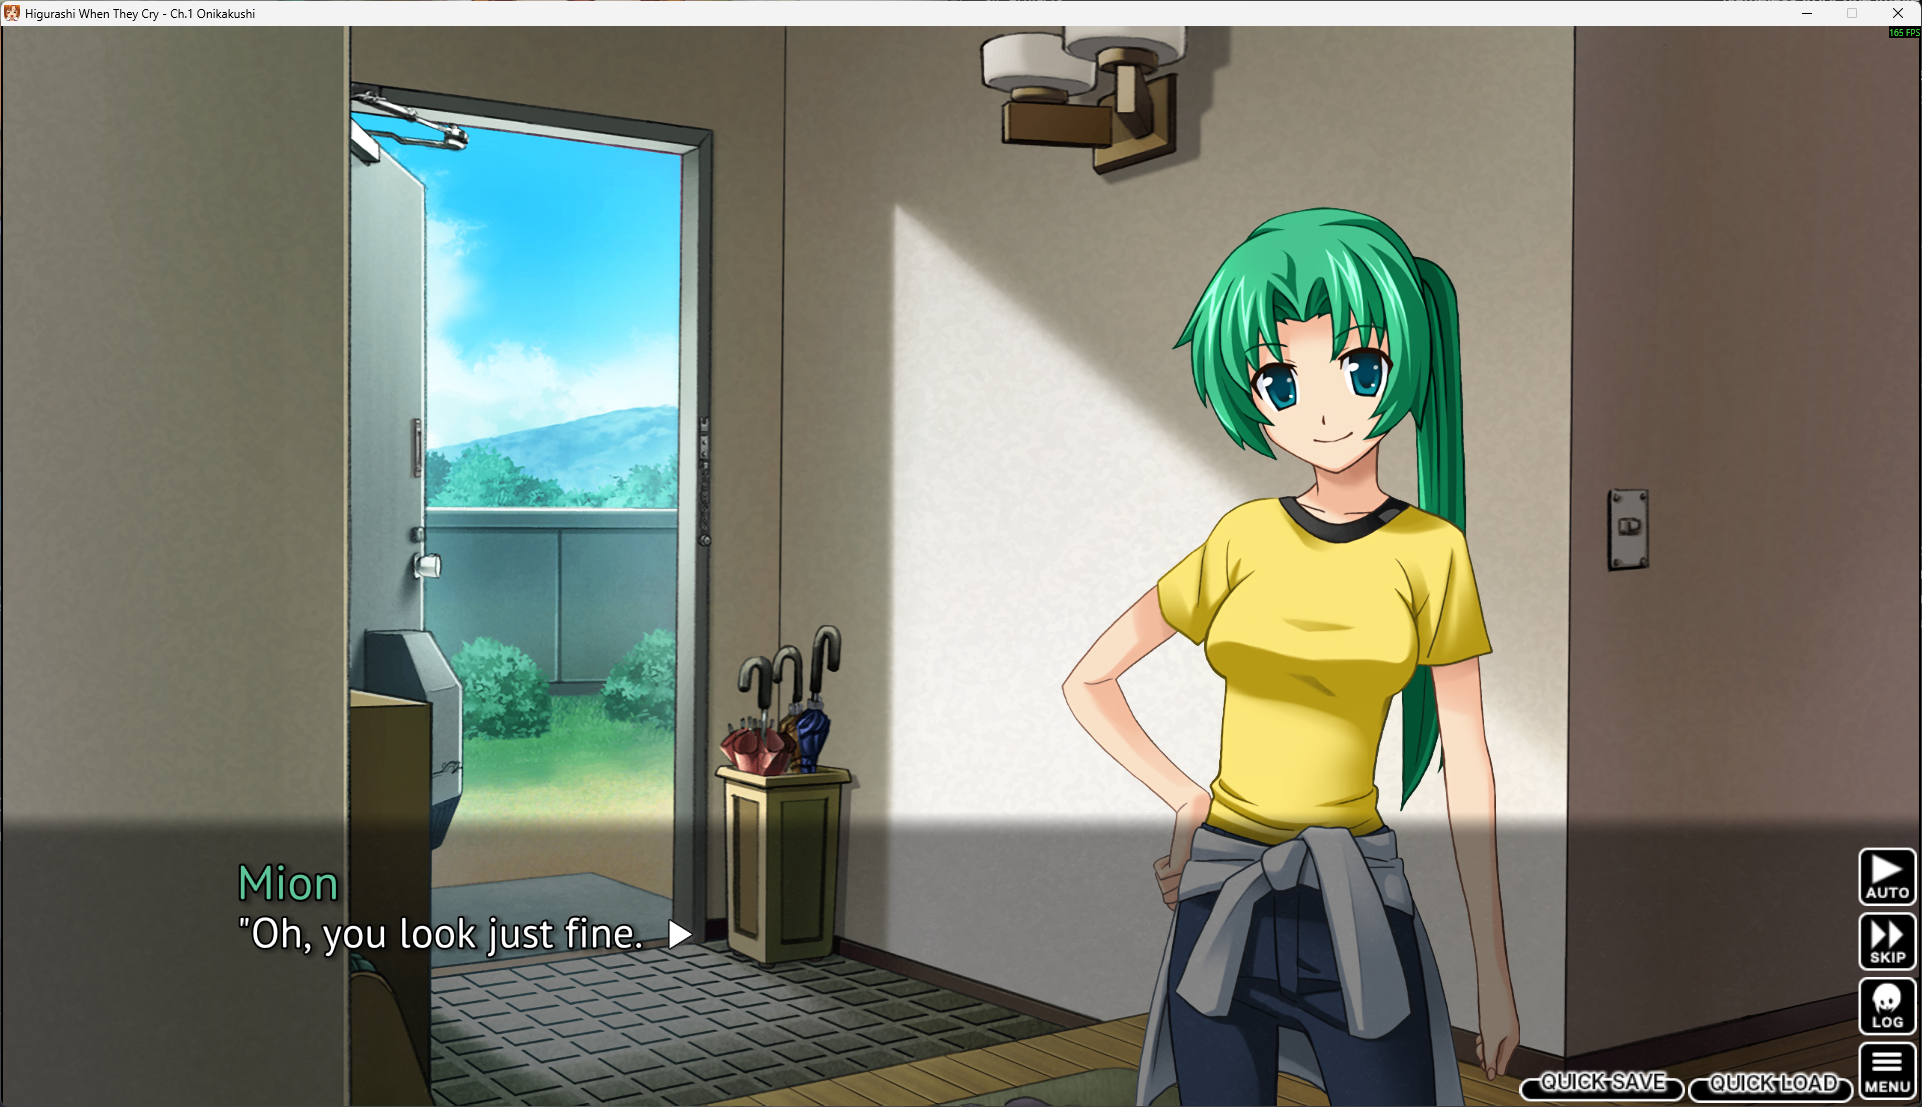
\includegraphics[width=0.9\linewidth]{img/higurashi_dialogue.png}
    \caption{Typical Visual Novel interface: background, character \textit{sprite}, and dialogue box \parencite{07th_expansion_higurashi_2015}}
    \label{fig:higurashi_dialogue}
\end{figure}

Camingue, Carstensdottir, and Melcer found that nine of the thirty academic definitions of the genre mention the presence of branching narration. These structures can lead to very different experiences: \textit{Steins;Gate 0} (2015) offers six different endings, while \textit{428: Shibuya Scramble} (2008) can lead to as many as 95 distinct conclusions. Conversely, 18\% of the titles surveyed contain no narrative branching at all. \parencite{camingue_what_2021}

\clearpage

From a market perspective, the 2019-2024 period saw growth in the genre's popularity, driven by the rise of distribution platforms such as Steam and mobile app stores. On Steam, 17,446 games in the genre are listed in Switzerland\footnote{Number recorded directly on Steam in Switzerland on 29 April 2026 at 19:00.}; the genre enjoys a significant presence there, confirming the existence of an active market. According to a report by Verified Market Research, the global \gls{vn} market was valued at 139 million dollars in 2023 and is expected to reach 620 million dollars by 2031, representing a compound annual growth rate of 8.5\% over the 2024-2031 period. \parencite{noauthor_visual_nodate}

The scale of the genre is also reflected in the count kept by VNDB, a community-run database dedicated to \glspl{vn}. The platform currently lists 64,577 \glspl{vn}\footnote{Number recorded directly on vndb.org on 13 July 2026 at 01:20.}, covering both commercial productions and free or amateur works, on which 52,804 professionals (writers, directors, composers, among others) have been credited\footnote{Number recorded directly on vndb.org on 13 July 2026 at 01:20.}. VNDB also brings together a community of more than 632,000 registered users\footnote{Calculated from the pagination of the site's user list (6,327 pages of 100 users and 21 users on the last page), recorded on 13 July 2026 at 01:20.}. \parencite{vndb_visual_nodate}



\subsection{Existing Visual Novel Engines}
\label{sec:moteur_vn_existant}

Game engines are software tools designed to facilitate game creation, handling recurring technical aspects such as display, resource management, or interaction logic. In the \gls{vn} field, several such tools exist, each based on a different approach to interactive narration.



\subsubsection{Ren'Py}

Several \gls{vn} engines exist. Ren'Py is a \gls{vn} engine used by thousands of creators around the world, allowing interactive stories combining text, images, and sound to be told, on both computer and mobile. To date, Ren'Py has been used to create more than 8,000 \glspl{vn}, games, and other interactive works. \parencite{noauthor_renpy_nodate}

Ren'Py notably offers support for branching narratives, a save system, the ability to roll back within the story, a variety of scene transitions, video playback, and full interface customisation through its dedicated language, \textit{Screen Language}. Ren'Py scripts use a \gls{syntaxe} close to a screenplay format, while also allowing Python blocks to be included for users who want to add advanced features. \parencite{noauthor_renpy_nodate}

\clearpage

Kretzschmar and Raffel argue that Ren'Py's popularity stems from being free of charge, its \glsit{opensource} nature, and the extent of its documentation, which allows anyone to learn its finer points. \parencite{kretzschmar_history_2023}

However, Ren'Py has several limitations for the purposes of this project. Although the engine offers a web export option based on \gls{webassembly}, this feature requires a compilation step through the software's interface, followed by manually uploading the generated files to a compatible host. In addition, the engine's official documentation flags significant restrictions tied to this export: no support for \textit{multi-threading}\footnote{\textbf{Multi-threading}: a program's ability to execute several instruction sequences in parallel, on separate processor cores. \parencite{noauthor_javascript_2026}}, no ability to make network requests from the browser, and file-size constraints imposed by hosting providers. \parencite{noauthor_renpy_nodate}



\subsubsection{Twine}

Twine is a free, open tool for creating non-linear interactive stories in hypertext form: the author links fragments of text, called passages, by means of links, with no programming knowledge required for this basic structure. \parencite{klimas_introduction_nodate}

This approach differs from that of the \gls{vn} engines presented above. Where Ren'Py or the engine developed in this project rely on a script or \gls{schema} file that linearly describes scenes, characters, and dialogue, Twine organises the narrative as a graph of interconnected passages, a structure closer to text-based interactive fiction than to a \gls{vn} in the strict sense, which implies visual staging (backgrounds, \glspl{sprite}, dialogue box). To go beyond a simple hyperlink, for instance to handle variables or conditional logic, the author must use the macro language specific to the chosen story format, which represents an additional learning step compared with simply creating links. \parencite{klimas_introduction_nodate}

Twine is thus a relevant point of comparison for this project: like \nsit, the tool runs in the browser and allows a story to be published as a self-contained file, with no compilation step imposed on the author. It differs, however, in its model for structuring the narrative, based on the hyperlink rather than a declarative data \gls{schema}, and in the absence of integrated visual staging comparable to that of a \gls{vn}.

\clearpage


\subsection{No-code/Low-code Approaches}

\textit{\glsdisp{nocode}{No-code}} platforms allow applications to be created with no programming knowledge, through visual tools, predefined templates, and ready-to-use logic blocks. \textit{\glsdisp{nocode}{Low-code}} tools, on the other hand, allow code to be added for greater control, while remaining accessible to non-developers.

Concretely, \textit{\glsdisp{nocode}{no-code}} platforms rely on drag-and-drop interfaces, prefabricated resources, and visual scripting. \textit{GDevelop}, \textit{Buildbox}, and \textit{Construct} can be cited as representative examples. \textit{\glsdisp{nocode}{Low-code}} tools, such as \textit{Unity's Bolt}, \textit{Unreal Engine's Blueprints}, or \textit{GameMaker Studio}, offer templates and simplified scripting options, with greater flexibility. \parencite{labs_rise_2024}

These approaches are of growing interest in the independent video game industry. Low production costs and the accessibility of development tools have allowed many independent developers to enter the market, leading to an increase in the number of diverse and innovative titles. \parencite{noauthor_visual_nodate}

However, these tools remain mostly tied to graphical interfaces and desktop environments. Writing a story directly as structured text, without going through a visual interface, remains an approach that is little explored in the current ecosystem.



\subsection{Data Description Formats: Comparison and Choice}

To meet the goal of an entirely text-based creation process, the choice of data format is decisive. Several text-based formats are used today to structure data that is readable by humans and interpretable by a machine.


\subsubsection{YAML}

\gls{yaml} is an indentation-based format, known for its readability. However, this readability comes at a cost: its \gls{syntaxe} is sensitive to spacing and special characters, which can produce silent errors that are difficult for a non-developer user to diagnose. In addition, native \glspl{parseur} for \gls{yaml} are not built into web browsers, which would require adding an external dependency to the project. \parencite{noauthor_-_nodate}

\clearpage


\subsubsection{TOML}

\gls{toml} is a format designed for configuration files, clear and explicit in its \gls{syntaxe}. It is, however, less suited to representing the deep hierarchical structures and nested arrays characteristic of a branching scenario. \parencite{noauthor_toml_nodate}


\subsubsection{Ink}

Ink, developed by Inkle Studios, is a narrative scripting language specifically designed for interactive fiction. Its \gls{syntaxe} is expressive and close to natural language, which makes it appealing to authors. However, it requires a dedicated execution engine (the Inkle \glsit{runtime}), which adds an external dependency, and its structure remains a full-fledged programming language, learning which goes beyond the scope of a simple data format. \parencite{noauthor_ink_nodate}


\subsubsection{JSON}

\gls{json} is an open file and data-interchange format that uses human-readable text to store and transmit data objects as key-value pairs and arrays. Although derived from \gls{js}, \gls{json} is independent of any programming language: most modern languages include native tools for generating and parsing data in \gls{json} format. \parencite{noauthor_what_nodate}

For this project, \gls{json} offers several advantages. Its key-value \gls{syntaxe} is intuitive, readable in any text editor, and requires no specialised tool to write. It is thus a natural choice for allowing an author, even without advanced technical skills, to describe a story in a structured way. In addition, \gls{json} is natively supported by \gls{js} and is therefore directly interpretable in a browser with no additional dependency, unlike \gls{yaml} or Ink.

An inherent risk with \gls{json} lies in its sensitivity to \gls{syntaxe} errors: a missing comma or an unclosed quotation mark makes the file invalid. This risk is mitigated in this project by the use of the \gls{zod} \gls{librairie}, which allows not only the file's \gls{syntaxe} but also the conformance of its structure to the \gls{schema} expected by the engine to be validated at runtime, with explicit error messages.

% ================
% Autres chapitres
% ================

\section{Méthodologie}
\label{chap:methodologie}

\subsection{Vue d'ensemble}

Je structure ce projet comme un développement itératif, plutôt que comme une réalisation linéaire. L’idée est de construire une première base fonctionnelle, puis d’ajuster progressivement le moteur en fonction des contraintes rencontrées: techniques, de format et de temps. Cette manière de faire me paraît plus adaptée à un projet de ce type, parce qu’elle permet de vérifier rapidement ce qui fonctionne réellement avant d’aller plus loin.

Le processus global repose sur trois axes: un cycle de développement basé sur le modèle \glsit{pdca}, une priorisation claire des fonctionnalités dont les objectifs sont définis au chapitre \ref{sec:objMediaProject}, et une validation fonctionnelle à chaque itération. Cette structure sert de fil conducteur tout au long du projet.


\subsection{Cycle de développement itératif (PDCA)} \label{sec:PDCA}

Le modèle \glsit{pdca} (\textit{Plan}, \textit{Do}, \textit{Check}, \textit{Act}), formalisé par W. Edwards Deming dans le cadre de l'amélioration continue des processus \parencite{deming_out_1986}, constitue le cadre méthodologique de ce projet. Je retiens ce modèle parce qu’il colle bien à un travail de développement où les décisions doivent être revues au fur et à mesure. Chaque itération suit donc les quatre phases décrites dans le tableau \ref{tab:defPDCA}.

\begin{table}[H]
    \centering
    \caption{Définition du cycle PDCA utilisée}
    \renewcommand{\arraystretch}{1.5}
    \begin{tabular}{p{1.5cm} p{11cm}}
        \hline
        \textbf{Nom} & \textbf{Description} \\
        \hline
        \textbf{Plan} & Définition des fonctionnalités à implémenter pour l'itération, en référence aux objectifs établis au chapitre. \\
        \addlinespace
        \textbf{Do} & Implémentation des fonctionnalités planifiées. \\
        \addlinespace
        \textbf{Check} & Évaluation du résultat par vérification fonctionnelle manuelle et, le cas échéant, par validation automatique via le \gls{parseur} \gls{zod}. \\
        \addlinespace
        \textbf{Act} & Ajustement des objectifs de l'itération suivante en fonction des écarts constatés. \\
        \hline
    \end{tabular}
    \label{tab:defPDCA}
\end{table}

Ce modèle est retenu pour sa capacité à intégrer les retours d’évaluation sans devoir redéfinir l’ensemble du périmètre à chaque étape.

\clearpage

Le développement se déroule en trois étapes successives, dont les objectifs sont résumés dans le tableau \ref{tab:objectifs_iterations} et décrits en détail au chapitre \ref{chap:MediaProject}. Je choisis de les distinguer clairement pour rendre l’évolution du projet plus lisible.

\begin{table}[H]
    \centering
    \caption{Objectif par itération}
    \renewcommand{\arraystretch}{1.5}
    \begin{tabular}{p{0.5cm} p{2.7cm} p{9.5cm}}
        \hline
        \textbf{N°} & \textbf{Objectif} & \textbf{Description} \\
        \hline
        1 & Fonctionnement du moteur & Implémentation des mécaniques fondamentales (affichage du texte, gestion des scènes, gestion des choix) et vérification du comportement attendu dans le navigateur. \\
        \addlinespace
        2 & Optimisation & Amélioration des performances internes, notamment par l'utilisation de \glspl{webworker} pour déléguer certains traitements hors du fil d'exécution principal, et refactorisation du code pour en augmenter la maintenabilité. \\
        \addlinespace
        3 & Sécurité et robustesse & Intégration de la \gls{librairie} \gls{zod} pour valider à l'exécution la conformité des fichiers \gls{json} au \gls{schema} attendu, et pour avertir l'utilisateur en cas de fichier de sauvegarde corrompu ou invalide. \\
        \hline
    \end{tabular}
    \label{tab:objectifs_iterations}
\end{table}

\clearpage


\subsection{Critères d'évaluation et validation fonctionnelle}

En l’absence de tests automatisés formels, je valide chaque fonctionnalité à partir de deux approches complémentaires.


\subsubsection{Vérification fonctionnelle manuelle}

Chaque fonctionnalité implémentée est testée directement dans le navigateur, en condition réelle, à partir de fichiers \gls{json} représentatifs. Les cas de test couvrent à la fois des scénarios valides et des scénarios d'erreur intentionnellement construits (\glsit{negativetesting}): suppression de virgules ou de guillemets pour casser la \gls{syntaxe} \gls{json}, omission de champs obligatoires attendus par le moteur (comme le nom du personnage parlant), et injection de valeurs de mauvais type (par exemple, un booléen à la place d'une chaîne de caractères). Ces fichiers de tests sont disponibles dans le dépôt GitHub\footnote{\textbf{GitHub}: plateforme d'hébergement de code source et de gestion de versions basée sur \gls{git}. \parencite{noauthor_build_nodate}} du projet: \nsrepo. Le critère de validation est la conformité du comportement observé avec le comportement attendu défini lors de la phase \textit{Plan} de chaque itération.


\subsubsection{Validation par Zod} \label{sec:zod}

La \gls{librairie} \gls{zod}, intégrée lors de la troisième itération, valide à l'exécution la structure du fichier \gls{json} fourni par l'auteur. En cas d'écart par rapport au \gls{schema} défini: champ manquant, type incorrect, structure invalide, \gls{zod} retourne un message d'erreur explicite indiquant précisément la source du problème, ce qui constitue un mécanisme de détection d'erreurs déterministe.

\clearpage


\subsection{Considérations sur la sécurité et la robustesse}

Deux préoccupations guident les décisions de développement au-delà de la simple fonctionnalité.


\subsubsection{Robustesse du code}

L'utilisation de \gls{ts} comme surcouche typée de \gls{js} permet de détecter à la compilation un ensemble d'erreurs de type qui seraient silencieuses en \gls{js} pur. Combiné à la validation \gls{zod} à l'exécution, ce dispositif forme une double barrière contre les états invalides du moteur. \parencite{noauthor_starting_nodate}


\subsubsection{Sécurité du code}

Le moteur opère entièrement côté client, dans le navigateur, sans serveur \glsit{backend}. Cette architecture supprime une surface d'attaque importante: il n'y a ni base de données exposée, ni gestion d'authentification, ni transmission de données utilisateur vers un serveur tiers. Le contenu narratif est statique et ne transite pas par un serveur applicatif. La validation des fichiers de sauvegarde par \gls{zod} permet par ailleurs d'empêcher l'injection de données malformées susceptibles de mettre le moteur dans un état indéterminé.


\subsection{Objectifs du Media Project} \label{sec:objMediaProject}

L'objectif principal de ce projet est d'offrir une alternative entièrement textuelle aux moteurs de \gls{vn} existants, facile à utiliser et à mettre en ligne. Contrairement aux solutions actuelles présentées au chapitre \ref{sec:moteur_vn_existant}, telles que Ren’Py, qui nécessite l'installation d'un environnement de développement dédié, ou Twine, dont la structure hypertextuelle impose l'apprentissage d'un langage de macros propre pour dépasser le simple lien, \nsits permet à tout auteur disposant de connaissances de base en \gls{json} de créer et de publier un \gls{vn} fonctionnel.

En proposant une solution \glsit{opensource}, le projet laisse la possibilité aux personnes possédant des connaissances en développement de modifier et d'étendre les fonctionnalités selon leurs besoins. L'\glsit{opensource} permet également à toute personne intéressée de contribuer activement au développement du moteur.

\clearpage

Le tableau \ref{tab:objectifs_moscow} définit les objectifs selon la méthode de priorisation \glsit{moscow} \parencite{clegg_case_1994}.

\begin{table}[H]
    \centering
    \caption{Objectifs du Media Project selon la priorisation MoSCoW}
    \renewcommand{\arraystretch}{1.5}
    \begin{tabular}{p{2cm} p{4.5cm} p{6cm}}
        \hline
        \textbf{Priorité} & \textbf{Fonctionnalité} & \textbf{Description} \\
        \hline
        Must & Effet machine à écrire & Affichage du texte caractère après caractère, simulant une machine à écrire. \\
        \addlinespace
        Must & Gestion des scènes & Navigation entre scènes, permettant les changements de décor et la progression narrative. \\
        \addlinespace
        Must & Gestion des choix & Présentation de choix au joueur, orientant la narration vers des routes différentes. \\
        \addlinespace
        Should & Gestion des saisies & Stockage d'une valeur saisie par le joueur, réutilisable dans le récit via une clé. \\
        \addlinespace
        Can & Fonctionnalités additionnelles & Toute autre fonctionnalité envisageable selon le temps disponible (sons, images, transitions). \\
        \hline
    \end{tabular}
    \label{tab:objectifs_moscow}
\end{table}

\clearpage


\subsection{Limites méthodologiques}

Cette approche présente deux limites principales. La première concerne l'absence de tests automatisés (\textit{unit tests}\footnote{\textbf{Test unitaire} (\textit{unit test}): test automatisé vérifiant le comportement d'une unité de code isolée. (\cite{beck_test-driven_2002};\cite{aniche_effective_2022})}, \textit{integration tests}\footnote{\textbf{Test d'intégration} (\textit{integration test}): test automatisé vérifiant que plusieurs unités ou composants fonctionnent correctement ensemble. \parencite{aniche_effective_2022}}). Le développement privilégie la mise en fonctionnement progressive des fonctionnalités sur la mise en place d'une suite de tests formelle. Cette absence implique que la couverture des cas limites dépend de l'exhaustivité des tests manuels réalisés et que des régressions introduites lors d'une itération pourraient passer inaperçues.

La seconde limite concerne l'absence de validation par des professionnels du secteur. Depuis janvier 2026, je contacte des développeurs de \gls{vn}, dans le but de recueillir leur avis sur l'approche retenue pour faciliter le développement de \gls{vn}, ainsi que des développeurs web, dans le but de discuter de l'infrastructure mise en place pour faire fonctionner le moteur. Ces sollicitations restent, à ce jour, sans réponse. En l'absence de retour de professionnels, l'évaluation du projet repose donc uniquement sur une validation interne au moyen d'un \glsit{poc} fonctionnel, sans confrontation à un regard extérieur spécialisé. Ces deux limites seront reprises dans l'évaluation critique au chapitre \ref{chap:resultats}.

\section{Implementation}
\label{chap:MediaProject}

This part forms the core of the work. Here I present the design and development of \textbf{\ns}, an \glsit{opensource} \gls{vn} engine entirely driven by text files in \gls{json} format. The author writes their story in a \gls{json} file that conforms to the defined \gls{schema}, then puts the project online either by compiling the \gls{reactjs} application into static files via \texttt{npm run build}, or through a continuous integration platform such as Vercel\footnote{\textbf{Vercel}: cloud deployment platform specialised in static web applications and \gls{js} frameworks. It automates building and deployment on every change to the source repository. \parencite{noauthor_vercel_nodate}} or GitHub Pages\footnote{\textbf{GitHub Pages}: static hosting service built into GitHub, allowing a repository's content to be automatically published as a website accessible via a public URL, with no server configuration. \parencite{noauthor_documentation_nodate}}. The final \gls{vn} thus remains accessible from any modern web browser, with no installation required on the player's side. The project's source code is publicly available on GitHub at the following address: \nsrepo.

The development followed an iterative logic: each iteration corresponded to a set of features that were implemented, tested, and evaluated before moving on to the next step.


\subsection{Scope Evolution: From Library to Application}

Initially, I had planned to develop \nsits as a \gls{reactjs} \gls{librairie} publishable on \gls{npm}, integrable by a third-party developer through a simple install command. The idea was to distribute the engine as a reusable component, independent of any host application.

To learn how to implement this architecture, two resources were consulted: a 2024 YouTube playlist by Imran Hussain (username \textit{Imran Codes}), titled \textit{Building a React Component Library: A Senior Developer's Guide}\parencite{imran_codes_1_2024} (targeting \gls{reactjs} 16), and a text article by Alex Eagleson published on dev.to in November 2021 and updated in December 2022 \parencite{noauthor_how_2021} (targeting \gls{reactjs} 17 and rollup\footnote{\textbf{Rollup}: \gls{js} bundling tool specialised in building distributable \gls{librairie}s. In \textit{\gls{librairie} mode}, it compiles the source code into one or more optimised files, together with \gls{ts} type definitions, ready to be published as an \gls{npm} \glsit{package}. \parencite{noauthor_introduction_nodate}} V2). Both resources relied on the same approach: configuring rollup in \gls{librairie} mode via a \texttt{rollup.config.js} file, combining the \texttt{@rollup/plugin-typescript}, \texttt{@rollup/plugin-commonjs}, and \texttt{rollup-plugin-dts} \glspl{plugin}.

\clearpage

In both cases, the \glsit{build} command (\texttt{npm run build}) failed. The errors encountered stemmed from the rollup configuration, whose requirements changed across successive versions of the tool. Eagleson's article itself flags this problem: a note embedded in the text indicates that some tools have been updated and that the instructions as written no longer work. \parencite{noauthor_how_2021} The comments on both resources, also roughly a year old, offered partial fixes that did not resolve the problem in the context of \gls{reactjs} 19 and current versions of rollup.

No more recent resource based on a configuration adapted to \gls{reactjs} 19 could be identified; the available tutorials all used the same configuration approach, which has become incompatible with current versions of the tooling. It cannot be ruled out that some of the errors encountered resulted from a misinterpretation of the configuration steps on my part; this possibility cannot be excluded.

Faced with these obstacles and the project's time constraints, the decision was made to redirect the architecture toward a standalone \gls{reactjs} application. This more directly manageable approach achieves the project's main objective: making \gls{vn} creation accessible via the web, without requiring the distribution of an \gls{npm} \glsit{package}.

\clearpage


\subsubsection{Technical Stack and Tools}

The development of \nsits relies on the technologies and tools listed in Table \ref{tab:stack}.

\begin{table}[H]
    \centering
    \caption{Technical stack and tools used}
    \renewcommand{\arraystretch}{1.5}
    \begin{tabular}{p{4cm} p{9cm}}
        \hline
        \textbf{Tool / Technology} & \textbf{Role in the project} \\
        \hline
        \gls{reactjs} & \Gls{librairie} \gls{js} used to render the engine in the browser. \\
        \addlinespace
        \gls{vite} & \Glsit{build} tool and development server, enabling fast hot-reloading during development. \\
        \addlinespace
        \gls{ts} & Typed superset of \gls{js}, used to strengthen code robustness and make it easier to catch errors before runtime. \\
        \addlinespace
        \gls{json} & Format used to describe narrative content, serving as the engine's single source of truth \\
        \addlinespace
        GitHub & Source code hosting and version control platform, via \gls{git}. \\
        \hline
    \end{tabular}
    \label{tab:stack}
\end{table}

\clearpage


\subsubsubsection{React.js Optimisation Mechanisms} \label{sec:optim_react}

\gls{reactjs} offers several mechanisms for reducing the number of unnecessary \glspl{rendu} and improving an application's performance. Three of them were used in this project \parencite{noauthor_reference_nodate}:

\texttt{React.memo} is a function that \glslink{override}{short-circuits} a component's \gls{rendu} if its \texttt{props}\footnote{\textbf{Props} (\textit{properties}): in \gls{reactjs}, a read-only object passed to a component by its parent component to configure its display or behaviour. \parencite{noauthor_reference_nodate}} have not changed since the previous \gls{rendu}. Without this mechanism, any state change in a parent component triggers the recomputation of all of its child components, whether or not they are affected by the change.

\texttt{useMemo} is a \glsit{hook} in \gls{reactjs} that caches the result of an expensive computation between two \glspl{rendu}. The computation is only rerun if one of its declared dependencies has changed, avoiding unnecessary recomputation on every \gls{rendu}.

\texttt{useRef} is a \glsit{hook} that persists a value across \glspl{rendu} without triggering a \glslink{rendu}{re-render} when it changes. It is used to store references to \acrshort{dom} elements or internal values whose change should not trigger an interface update.


\subsubsection{Development Method}

Development followed an iterative process based on the \glsit{pdca} cycle (\textit{Plan, Do, Check, Act}), as defined in the methodology presented in Section \ref{sec:PDCA}. Each iteration corresponds to a full cycle: planning the features to implement, development, evaluation through functional tests, then deciding on the adjustments to make for the next iteration.

This model was chosen for its ability to continuously incorporate evaluation feedback, without needing to redefine the entire scope at each step.

\clearpage


\subsection{Constraints and Limitations}

\subsubsection{Deployment Constraint}

Unlike traditional game engines that compile the project into a native executable, \nsits relies on web technologies. To create a \gls{vn} with this engine, the author must download the project, then write their story in a \gls{json} file following the defined \gls{schema}. The result can then be put online in two ways:

\begin{itemize}
    \item By compiling the \gls{reactjs} application into static files via the \texttt{npm run build} command, then hosting those files on any web server or static host.
    \item By connecting the repository to a continuous integration platform such as Vercel or GitHub Pages, which automatically handles building and deployment on every change to the project.
\end{itemize}

In both cases, the final \gls{vn} is accessible from any modern web browser, with no installation required on the player's side; see Figure \ref{fig:deploiement-flux}.

\begin{figure}[H]
    \centering
    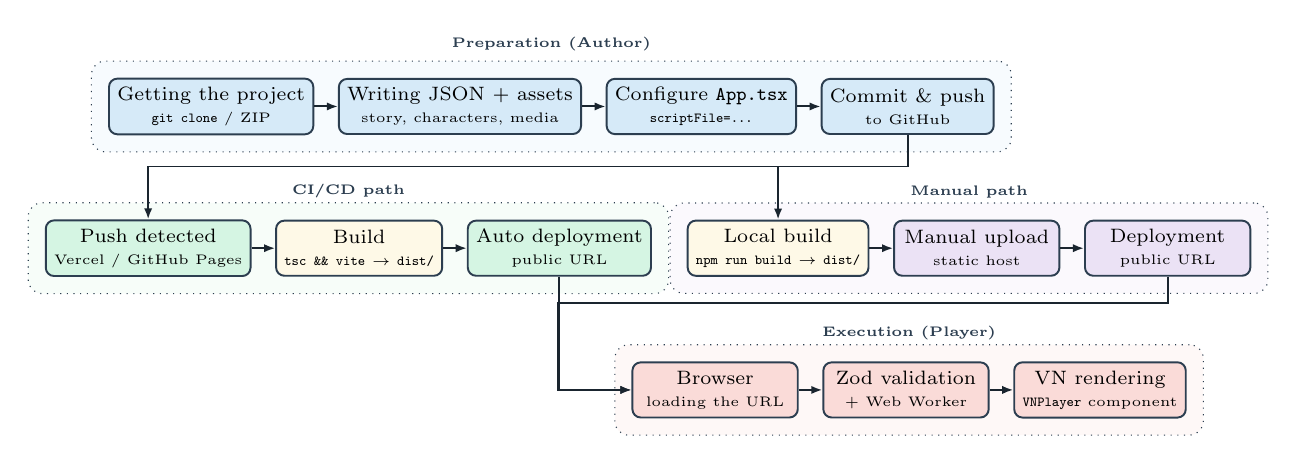
\begin{tikzpicture}[
        node distance = 0.3cm and 0.3cm,
        every node/.style = {font=\scriptsize, align=center},
        box/.style = {
            rectangle, rounded corners=3pt,
            draw=clrBorder, line width=0.7pt,
            minimum width=2.1cm, minimum height=0.7cm,
            inner sep=3pt
        },
        auteur/.style = {box, fill=clrAuteur},
        build/.style  = {box, fill=clrBuild},
        cloud/.style  = {box, fill=clrCloud},
        player/.style = {box, fill=clrPlayer},
        alt/.style    = {box, fill=clrAlt},
        arrow/.style  = {-{Latex[length=4pt,width=3pt]},
                         line width=0.7pt, color=clrArrow},
        lbl/.style    = {font=\tiny\itshape, color=clrNote},
    ]

%% ── Row 1: Preparation (Author) ─────────────────────────────────────────
\node[auteur] at (0,0) (dl)
    {Getting the project\\
     \tiny{\texttt{git clone} / ZIP}};

\node[auteur, right=of dl]      (content)
    {Writing JSON + assets\\
     \tiny{story, characters, media}};

\node[auteur, right=of content] (config)
    {Configure \texttt{App.tsx}\\
     \tiny{\texttt{scriptFile=...}}};

\node[auteur, right=of config]  (push)
    {Commit \& push\\
     \tiny{to GitHub}};

\draw[arrow] (dl)      -- (content);
\draw[arrow] (content) -- (config);
\draw[arrow] (config)  -- (push);

%% ── Row 2, left: CI/CD path ───────────────────────────────────────────
\node[cloud] at (-0.8,-1.8) (cicd)
    {Push detected\\
     \tiny{Vercel / GitHub Pages}};

\node[build, right=of cicd]     (buildci)
    {Build\\
     \tiny{\texttt{tsc \&\& vite} $\to$ \texttt{dist/}}};

\node[cloud, right=of buildci]  (deployci)
    {Auto deployment\\
     \tiny{public URL}};

\draw[arrow] (cicd)    -- (buildci);
\draw[arrow] (buildci) -- (deployci);

%% ── Row 2, right: Manual path ─────────────────────────────────────────
\node[build] at (7.2,-1.8) (buildman)
    {Local build\\
     \tiny{\texttt{npm run build} $\to$ \texttt{dist/}}};

\node[alt, right=of buildman]   (upload)
    {Manual upload\\
     \tiny{static host}};

\node[alt, right=of upload]     (deployman)
    {Deployment\\
     \tiny{public URL}};

\draw[arrow] (buildman) -- (upload);
\draw[arrow] (upload)   -- (deployman);

%% ── Arrows push → paths ────────────────────────────────────────────────────
\draw[arrow] (push.south) -- ++(0, -0.4cm) -| (buildman.north);
\draw[arrow] (push.south) -- ++(0,-0.4cm) -| (cicd.north);

%% ── Row 3: Execution (Player) ───────────────────────────────────────────
\node[player] at (6.4,-3.6) (browser)
    {Browser\\
     \tiny{loading the URL}};

\node[player, right=of browser] (zodwk)
    {Zod validation\\
     \tiny{+ Web Worker}};

\node[player, right=of zodwk]   (vn)
    {VN rendering\\
     \tiny{\texttt{VNPlayer} component}};

\draw[arrow] (deployci)  |- (browser.west);
\draw[arrow] (deployman) |- (4.4cm, -2.5cm) |- (browser.west);
\draw[arrow] (browser) -- (zodwk);
\draw[arrow] (zodwk)   -- (vn);

%% ── Grouping boxes ───────────────────────────────────────────────────
\begin{scope}[on background layer]
  \node[draw=clrBorder, dotted, rounded corners=5pt, fill=clrAuteur!20,
        fit=(dl)(content)(config)(push), inner sep=6pt,
        label={[font=\tiny\bfseries, text=clrBorder]above:Preparation (Author)}
       ] {};

  \node[draw=clrBorder, dotted, rounded corners=5pt, fill=clrCloud!20,
        fit=(cicd)(buildci)(deployci), inner sep=6pt,
        label={[font=\tiny\bfseries, text=clrBorder, yshift=-2pt]above:CI/CD path}
       ] {};

  \node[draw=clrBorder, dotted, rounded corners=5pt, fill=clrAlt!20,
        fit=(buildman)(upload)(deployman), inner sep=6pt,
        label={[font=\tiny\bfseries, text=clrBorder, yshift=-2pt]above:Manual path}
       ] {};

  \node[draw=clrBorder, dotted, rounded corners=5pt, fill=clrPlayer!20,
        fit=(browser)(zodwk)(vn), inner sep=6pt,
        label={[font=\tiny\bfseries, text=clrBorder, yshift=-2pt]above:Execution (Player)}
       ] {};
\end{scope}

    \end{tikzpicture}
    \caption{Deployment flow of \nsit, from local configuration to execution in the browser (Author 2026)}
    \label{fig:deploiement-flux}
\end{figure}

\clearpage

\subsubsection{Format Constraint}

A fundamental constraint of this project is making the narrative content readable and interpretable both by a human and by a machine. The \gls{json} format was chosen to meet this requirement: its key/value model is sufficiently structured to be parsed deterministically by the \gls{parseur}, while remaining accessible to a non-developer author willing to follow a documented \gls{schema}.

However, this constraint carries an inherent limitation: the absence of semantic interpretation of natural language means the author must strictly follow the defined \gls{syntaxe}. A structural error in the \gls{json} file can block the engine's execution. Handling these errors and giving the author clear feedback are therefore a robustness goal to be addressed across the iterations.


\subsubsection{Scope Constraint}

For time reasons, the engine's functional scope is limited to the core \gls{vn} mechanics, as defined in Table \ref{tab:objectifs_moscow}. Other features, such as background music, character images, or a save system, are identified as desirable, but are not part of this work's primary objectives.


\subsection{Development Stages}

The development of \nsits took place over three successive iterations, each following the \glsit{pdca} cycle defined in Section \ref{sec:PDCA}. The objectives of each iteration were defined beforehand according to the \glsit{moscow} prioritisation set out in Table \ref{tab:objectifs_moscow}, and adjusted based on the results observed at the end of each cycle.


\subsubsection{First Iteration: The Basics of a VN}


\subsubsubsection{Plan}

The objective of this first iteration was to implement the engine's core mechanics: progressive text display (typewriter effect), scene navigation, and dialogue choice handling. These three features correspond to the \textit{Must} requirements in Table \ref{tab:objectifs_moscow}. It also involved defining the structure of the \gls{json} \gls{schema} used as the content source, i.e. the node types the engine would need to be able to interpret: dialogue, choice, scenes, and characters.


\subsubsubsection{Do}

I started by creating the project. To do so, I needed to choose a language, a \glsit{framework}, and a structure. For the language, I chose \gls{ts}, to benefit from static typing that provides safety as early as the development phase, before runtime even begins. As for the \glsit{framework}, I hesitated with Next.js\footnote{\textbf{Next.js}: server-rendering-oriented \gls{reactjs} \glsit{framework}, developed by Vercel \parencite{noauthor_nextjs_nodate}}, but it would have been overkill for this project: \nsits requires no server-side processing (\textit{\glsit{backend}}), with everything computed in the \glsit{frontend}. I therefore chose \gls{reactjs}, a \gls{js} \gls{librairie} I was already familiar with and which is perfectly suited to building this component-based project, allowing each part of the code to be kept separate.

Even before starting to build a single component, I began thinking about the structure I wanted to use for the \gls{json} file that would hold the story. I wanted something customisable, to leave as much freedom as possible to people wanting to use this project. To achieve this, I had to separate out several elements, illustrated in Table \ref{tab:obj_json_schema}.

\begin{table}[H]
    \centering
    \caption{Separation of the JSON file's main elements}
    \renewcommand{\arraystretch}{1.5}
    \begin{tabular}{p{4cm} p{9cm}}
        \hline
        \textbf{Object} & \textbf{Description} \\
        \hline
        Settings & Definitions of the application's global default values: customisation of the title screen, the credits page, and display behaviour. These values can be \glslink{override}{overridden} locally at the dialogue level. \\
        \addlinespace
        Characters & The declaration of characters, so that all characters and their information live in a single place. \\
        \addlinespace
        The story & All the elements used to tell the story. \\
        \hline
    \end{tabular}
    \label{tab:obj_json_schema}
\end{table}

Why these choices? Why not put the characters inside the story? There are several answers to these questions. To begin with, it gives a simple, readable structure: everything is separated according to clear, distinct purposes: what helps the author (settings), what will be used repeatedly (characters), and the narrative itself. Characters, like variables, are likely to appear across many scenes. Centralising them thus avoids any repetition in the file.

\clearpage

Code listing \ref{lst:json_example} shows this separation in a short example.

\begin{listing}[H]
\begin{minted}{json}
{
    "settings": {
        "startingScene": "start",
        "textSpeed": 45
    },
    "characters": {
        "Alice": {
            "name": "Alice",
            "fullName": "Alice Wonderland",
            "color": "#e07ae0"
        }
    },
    "story": {
        "start": {
            "background": "bg.png",
            "dialogues": [
                {
                    "name": "Alice",
                    "text": "Hello, world."
                },
                {
                    "name": "Alice",
                    "text": "Where shall we go?",
                    "options": [
                        { "text": "The library", "next": "library" },
                        { "text": "The park", "next": "park" }
                    ]
                }
            ]
        }
    }
}
\end{minted}
\caption{Example JSON file structure (Author 2026)}
\label{lst:json_example}
\end{listing}

\clearpage

As the iterations progressed, the \gls{schema} would grow to offer more options. This approach makes the \gls{vn}'s entire visual rendering customisable directly from the \gls{json} file, with no need to modify the engine's code: each scene's background image (\texttt{background} key), the colour associated with each character, as well as the appearance of the title screen and the credits page, defined at the settings level (see Table \ref{tab:obj_json_schema}). Font management via \acrshort{css} variables, added during the third iteration, rounds out this visual customisation.

Once the structure was defined, I needed to start development. This meant deciding where to start, and I chose to begin with the basic visual components: the title screen, the credits screen, and a background image component.

Since the title page, the credits, and the scenes would all have background images, I decided to make it a fully separate component to avoid repetition.

The reason I started with the title and credits screens instead of the core of the project, the \gls{vn} itself, is that I wanted to first take care of the simple elements that were not going to change much. Once these screens were done, I could devote myself entirely to the \gls{vn}, knowing the other screens were already finished.

Once these elements were done, I started working on the component I consider the most important: text display, with the typewriter effect. To make this component more powerful, my intention was for it to be able to \glslink{parseur}{parse} \acrshort{html} tags and to support a pause \gls{syntaxe} to give the text more punch. I therefore built a text \gls{tokenisation} system. The idea is simple: before display, the raw text is split into units, \textit{tokens}, which can be either ordinary text, \acrshort{html} tags, or pause markers, as illustrated in Figure \ref{fig:tokenisation-flux}. This separation lets the typewriter effect animate only the visible characters, without treating tags as text to display. Without this intermediate step, displaying \texttt{<b>word</b>} character by character would have risked producing partial tags visible on screen, or malformed \acrshort{html}.

\begin{figure}[H]
    \centering
    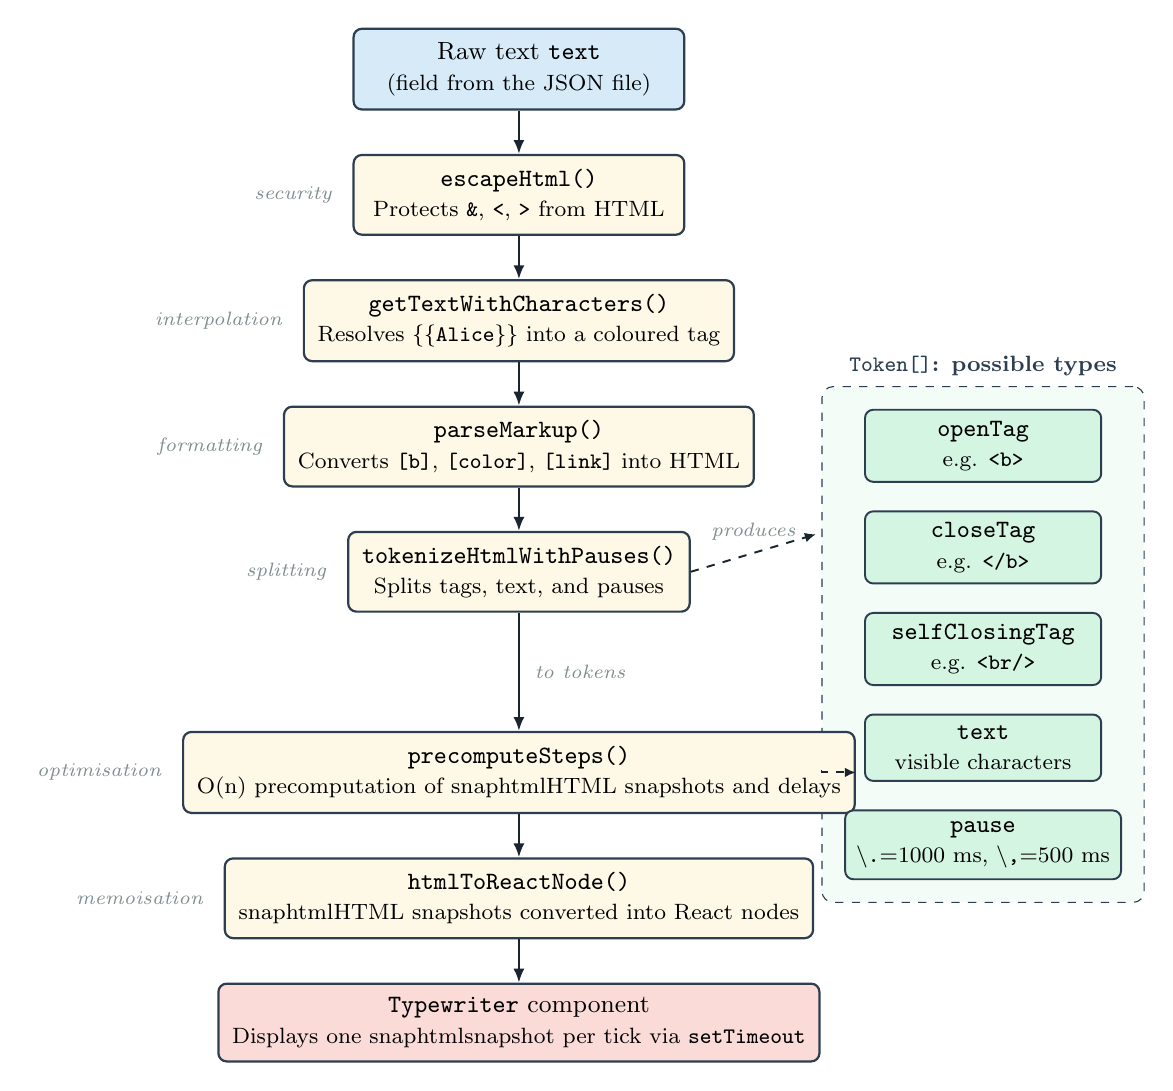
\begin{tikzpicture}[
    node distance = 0.55cm and 2.2cm,
    every node/.style = {font=\small, align=center},
    box/.style = {
        rectangle, rounded corners=3pt,
        draw=clrBorder, line width=0.8pt,
        minimum width=4.2cm, minimum height=0.9cm,
        inner sep=5pt
    },
    input/.style   = {box, fill=clrInput},
    process/.style = {box, fill=clrProcess},
    token/.style   = {rectangle, rounded corners=3pt,
                      draw=clrBorder, line width=0.7pt, fill=clrToken,
                      minimum width=3.0cm, minimum height=0.8cm,
                      inner sep=4pt, font=\small, align=center},
    output/.style  = {box, fill=clrOutput},
    arrow/.style   = {-{Latex[length=5pt,width=4pt]},
                      line width=0.8pt, color=clrArrow},
    darrow/.style  = {-{Latex[length=4pt,width=3.5pt]},
                      line width=0.7pt, color=clrArrow, dashed},
    lbl/.style     = {font=\scriptsize\itshape, color=clrNote}
    ]

%% ── Main column (left) ─────────────────────────────────────────

\node[input] (raw)
    {Raw text \texttt{text}\\
     \footnotesize{(field from the JSON file)}};

\node[process, below=of raw] (escape)
    {\texttt{escapeHtml()}\\
     \footnotesize{Protects \texttt{\&}, \texttt{<}, \texttt{>} from HTML}};

\node[process, below=of escape] (vars)
    {\texttt{getTextWithCharacters()}\\
     \footnotesize{Resolves \texttt{\{\{Alice\}\}} into a coloured tag}};

\node[process, below=of vars] (markup)
    {\texttt{parseMarkup()}\\
     \footnotesize{Converts \texttt{[b]}, \texttt{[color]}, \texttt{[link]} into HTML}};

\node[process, below=of markup] (tokenize)
    {\texttt{tokenizeHtmlWithPauses()}\\
     \footnotesize{Splits tags, text, and pauses}};

\node[process, below=1.5cm of tokenize] (precompute)
    {\texttt{precomputeSteps()}\\
     \footnotesize{O(n) precomputation of \glslink{snaphtml}{HTML snapshots} and delays}};

\node[process, below=of precompute] (react)
    {\texttt{htmlToReactNode()}\\
     \footnotesize{\glslink{snaphtml}{HTML snapshots} converted into React nodes}};

\node[output, below=of react] (render)
    {\texttt{Typewriter} component\\
     \footnotesize{Displays one \glslink{snaphtml}{snapshot} per tick via \texttt{setTimeout}}};

%% ── Vertical arrows ──────────────────────────────────────────────────────
\draw[arrow] (raw)        -- (escape);
\draw[arrow] (escape)     -- (vars);
\draw[arrow] (vars)       -- (markup);
\draw[arrow] (markup)     -- (tokenize);
\draw[arrow] (tokenize)   -- node[lbl, right=2pt] {to tokens} (precompute);
\draw[arrow] (precompute) -- (react);
\draw[arrow] (react)      -- (render);

%% ── Side annotations (left) ─────────────────────────────────────────
\node[lbl, left=4pt of escape]    {security};
\node[lbl, left=4pt of vars]      {interpolation};
\node[lbl, left=4pt of markup]    {formatting};
\node[lbl, left=4pt of tokenize]  {splitting};
\node[lbl, left=4pt of precompute]{optimisation};
\node[lbl, left=4pt of react]     {\gls{memoisation}};

%% ── Token table (right) ──────────────────────────────────────────────
\node[token, right=of tokenize, yshift= 1.6cm] (tok_open)
    {\texttt{openTag}\\
     \footnotesize{e.g. \texttt{<b>}}};

\node[token, below=0.35cm of tok_open] (tok_close)
    {\texttt{closeTag}\\
     \footnotesize{e.g. \texttt{</b>}}};

\node[token, below=0.35cm of tok_close] (tok_self)
    {\texttt{selfClosingTag}\\
     \footnotesize{e.g. \texttt{<br/>}}};

\node[token, below=0.35cm of tok_self] (tok_text)
    {\texttt{text}\\
     \footnotesize{visible characters}};

\node[token, below=0.35cm of tok_text] (tok_pause)
    {\texttt{pause}\\
     \footnotesize{\texttt{\textbackslash .}=1000 ms, \texttt{\textbackslash ,}=500 ms}};

%% Token bounding box
\begin{scope}[on background layer]
  \node[draw=clrBorder, dashed, rounded corners=4pt,
        fill=clrToken!25,
        fit=(tok_open)(tok_close)(tok_self)(tok_text)(tok_pause),
        inner sep=8pt,
        label={[font=\footnotesize\bfseries, text=clrBorder]above:\texttt{Token[]}: possible types}
       ] (tokbox) {};
\end{scope}

%% ── Arrows to/from the token table ────────────────────────────────
\draw[darrow] (tokenize.east)  -- ([xshift=-2pt, yshift=1.4cm]tokbox.west)
              node[midway, lbl, above=1pt] {produces};

\draw[darrow] ([yshift=-1.6cm]tokbox.west)  |- (precompute.east);

    \end{tikzpicture}
    \caption{Tokenization flow of the \texttt{Typewriter} component (Author 2026)}
    \label{fig:tokenisation-flux}
\end{figure}

Once all these elements were working, it was time for me to put in place the core logic of a \gls{vn}: navigation between dialogues and between scenes. I created a dialogue component, holding the text and, later, also the name of the speaking character. I also created the scene component, which brings together the text and the background image.

For interactivity, on a click or when the player presses \textit{Enter}, either the dialogue changes to the next one in the current scene, or, if we are at the scene's last dialogue, we are taken to the scene defined by that dialogue's \texttt{next} key, or to the credits page if that key is absent or if its value is \texttt{"\_\_end\_\_"}.

\clearpage

Another element I added was the ability to make choices. I made sure that buttons could appear on screen, letting the player choose which path to follow. Among the possible outcomes, the player can end up in another scene, at another dialogue of the current scene, or at a specific dialogue of another scene. The author can also choose to send the player to the credits page by setting \texttt{"\_\_end\_\_"} as the value of the \texttt{next} key.

Figure \ref{fig:NamelessStoryV1} presents the state of the engine at the end of this first iteration.\footnote{For legibility when printed, all engine screenshots shown in this chapter were taken with the browser zoom set to 175\%. The actual rendering, at the browser's default zoom (100\%), therefore displays elements proportionally smaller than those visible in these figures.\label{fn:zoom175}}

\begin{figure}[H]
    \centering
    \begin{subfigure}[b]{0.47\textwidth}
        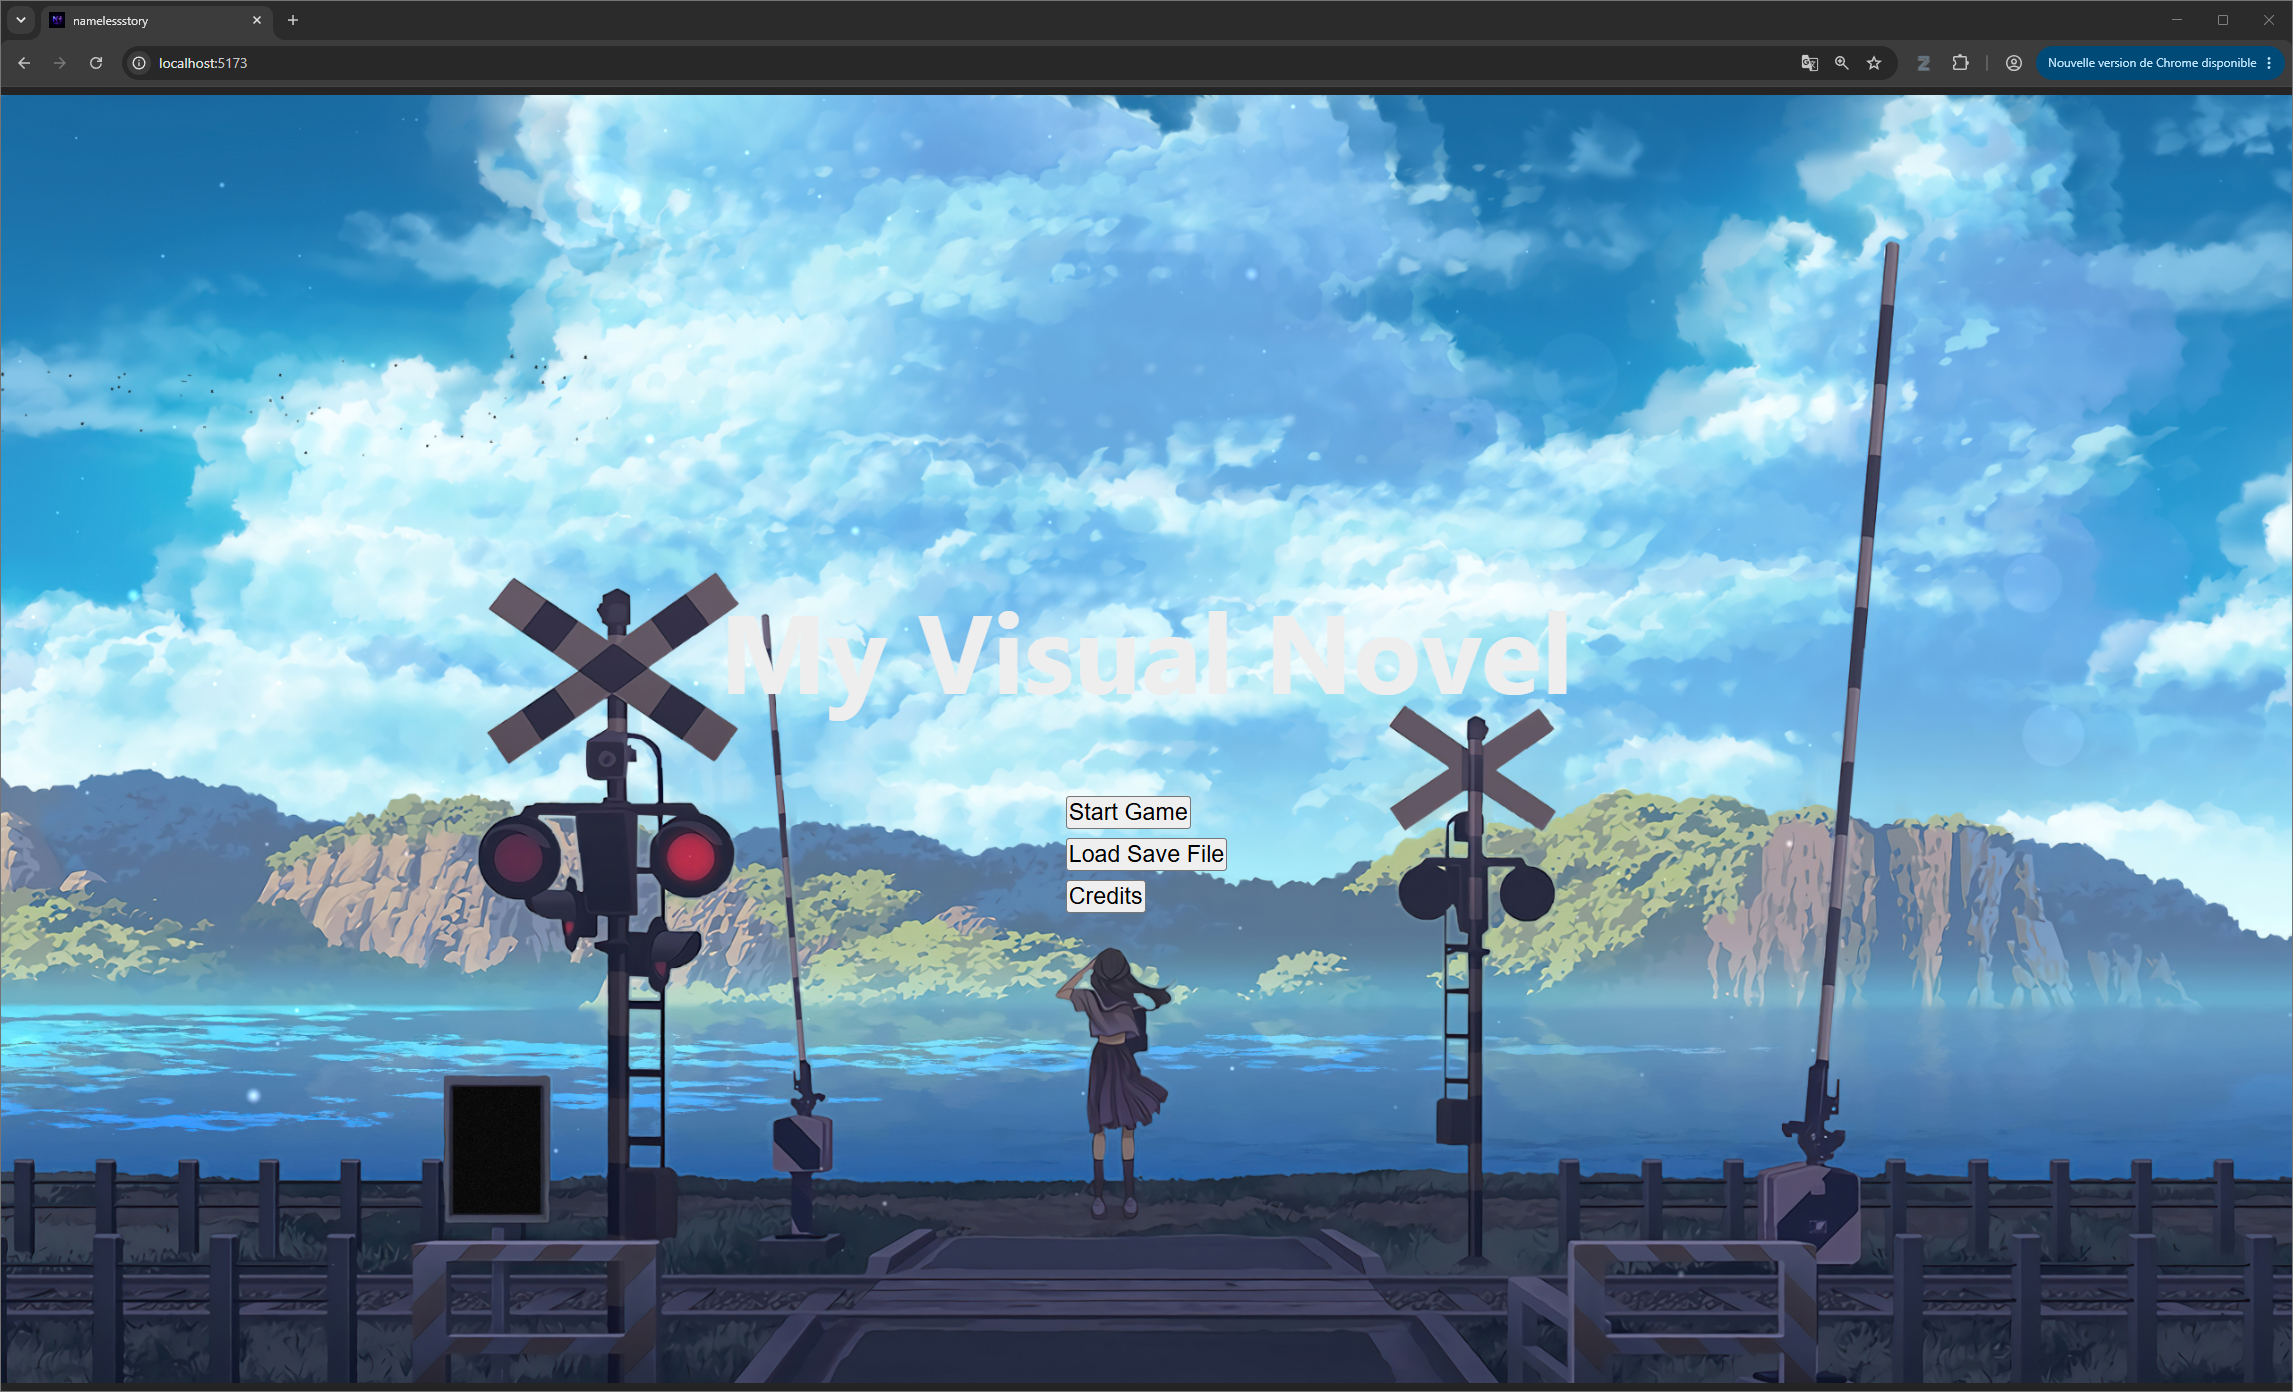
\includegraphics[width=\textwidth]{img/NamelessStory_V1_home.png}
        \caption{Title screen}
    \end{subfigure}
    \hfill
    \begin{subfigure}[b]{0.47\textwidth}
        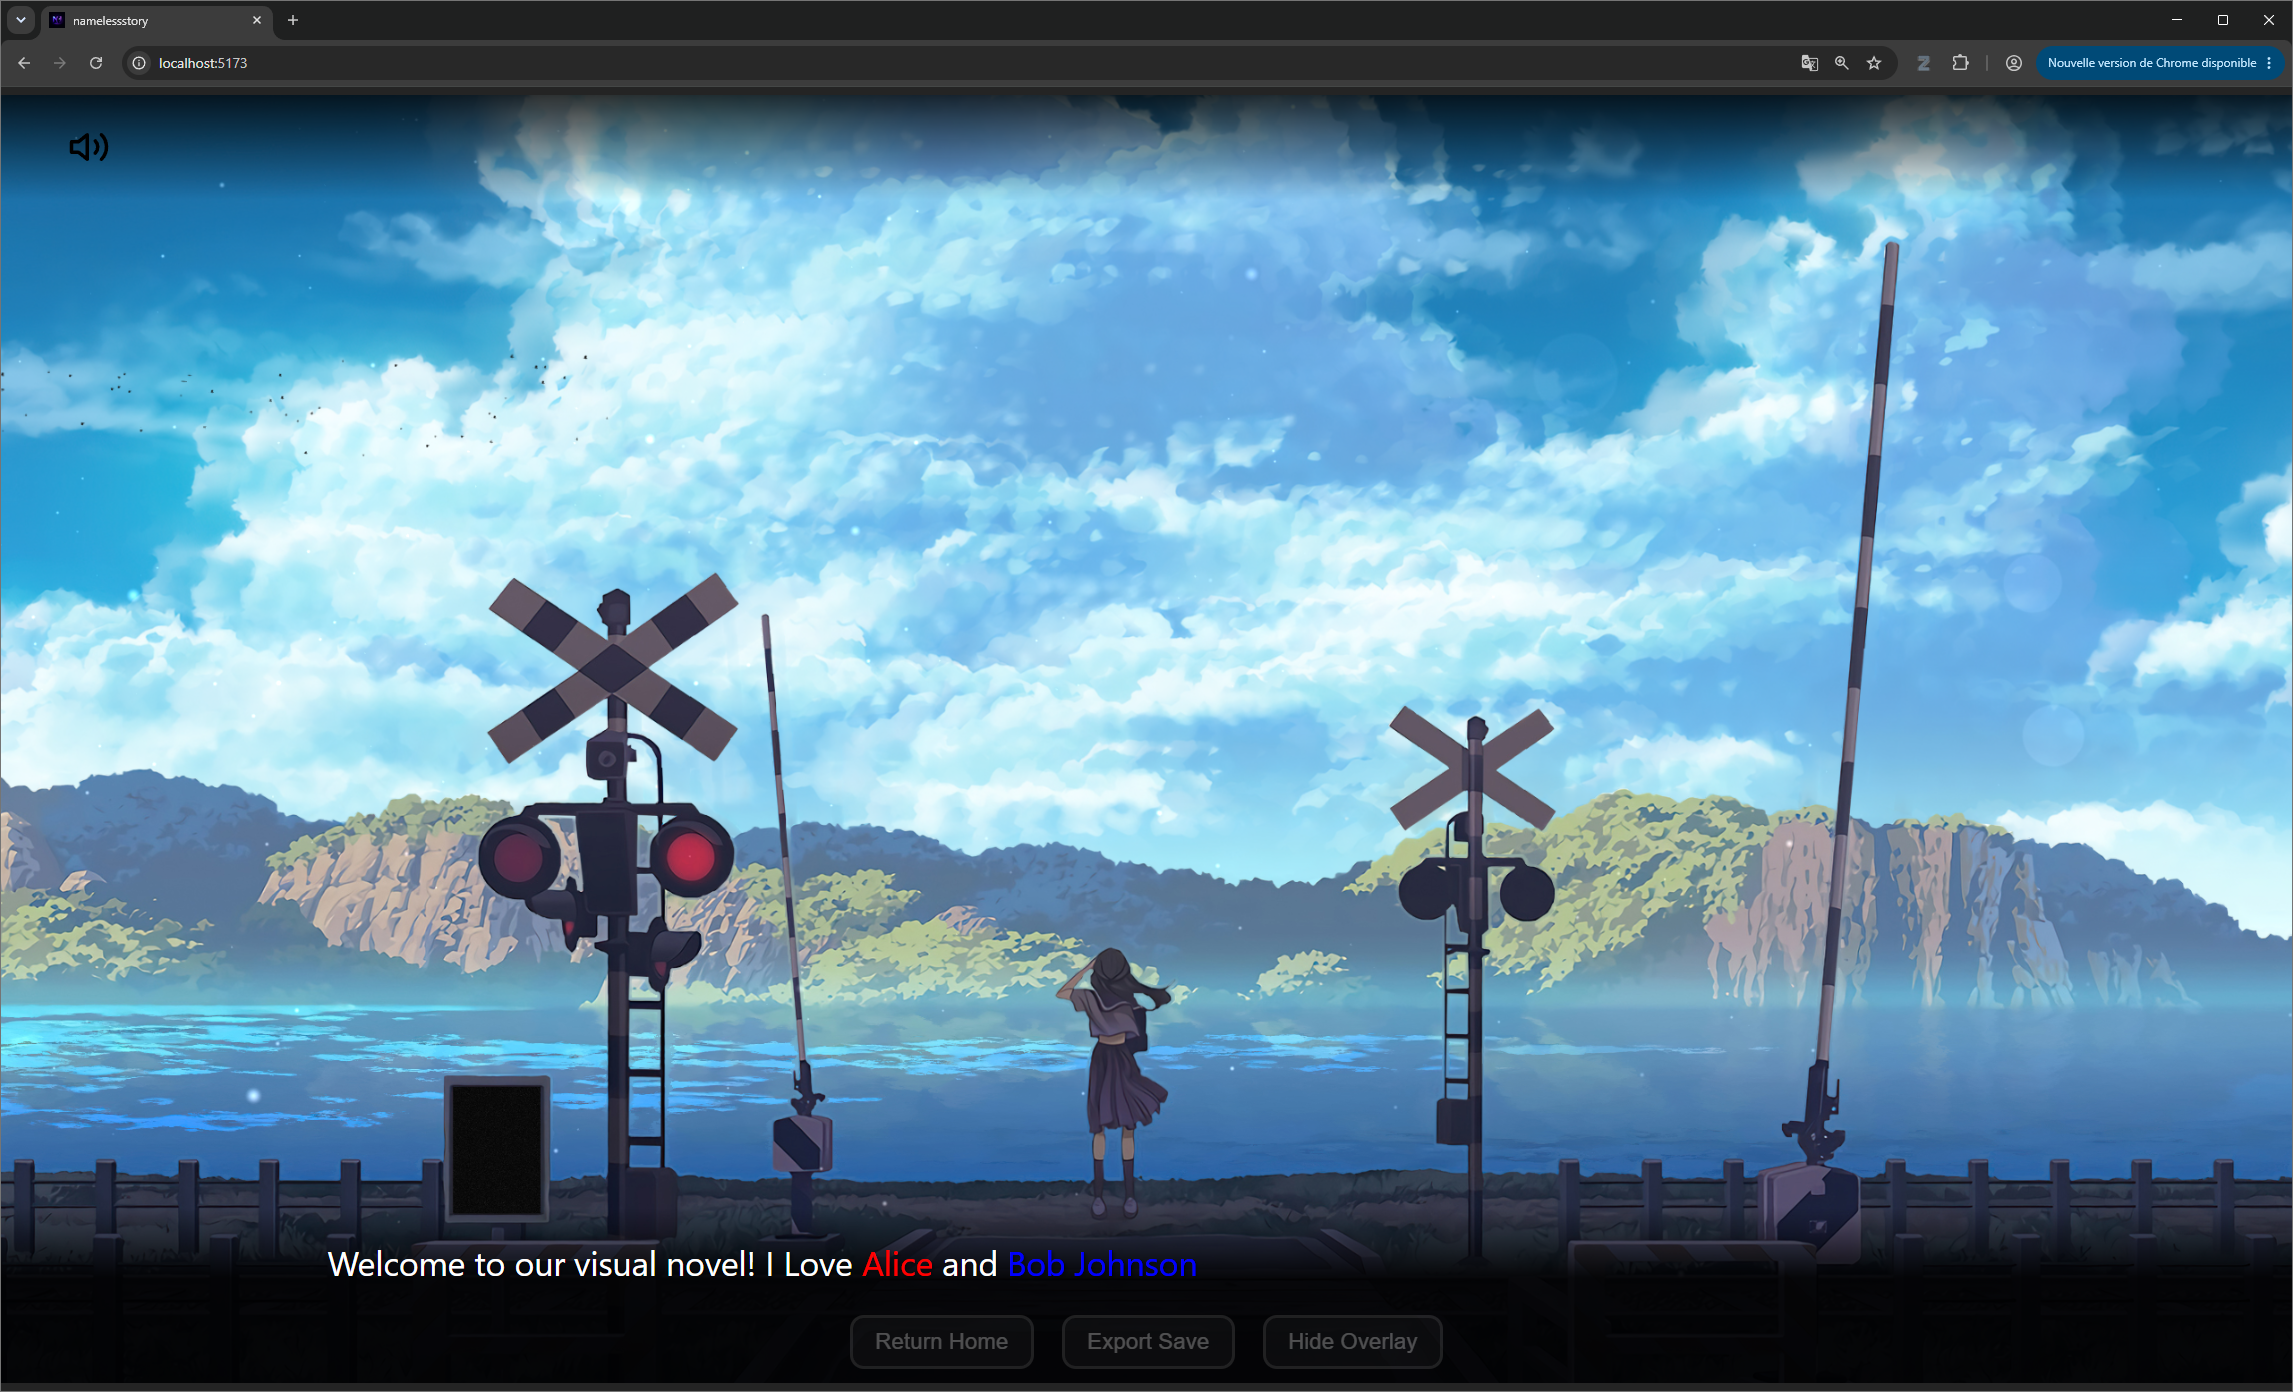
\includegraphics[width=\textwidth]{img/NamelessStory_V1_text.png}
        \caption{Dialogue display}
    \end{subfigure}
    \caption{\nsits at the end of the first iteration (Author 2026)}
    \label{fig:NamelessStoryV1}
\end{figure}

\clearpage


\subsubsubsection{Check}

At the end of this iteration, the core mechanics were functional and verifiable in the browser using a test \gls{json} file. Valid cases were tested manually: dialogue progression on click, navigation to another scene, display of choices, and option selection. Error scenarios were also intentionally constructed (\glsit{negativetesting}), notably by supplying structurally incomplete \gls{json} files, in order to check the engine's behaviour when faced with unexpected data.

These tests revealed that the engine exhibited undefined behaviour when faced with missing or erroneous data, without returning any actionable information to the author: no error message, no way to know what to fix.

Having focused mainly on functionality, the styling was still lacking. What mattered most to me at this stage of the project was having elements displayed on screen, not necessarily that they looked good.


\subsubsubsection{Act}

With a functional baseline in place, two options were open to me going forward: address the error-message problem or optimise the engine's performance. Not yet having the necessary knowledge of robustness and validation, I chose to focus on optimisation work, to ensure the engine avoided unnecessary recomputation and made efficient use of browser resources.

\clearpage


\subsubsection{Second Iteration: Optimisation}

\subsubsubsection{Plan}

The objective of this iteration was to improve the performance and maintainability of the code produced during the first iteration. In \gls{reactjs}, every state update on a parent component triggers a new \gls{rendu} of the entire tree of child components. In a \gls{vn} engine, where the global state changes with every line of dialogue, this behaviour can cause unnecessary recomputation of components whose data has not changed. A second focus concerned save handling: the operation of serialising the current state via \texttt{JSON.stringify()} was running on the browser's main thread. This is not a problem as long as the object to serialise stays modest in size. However, as the state grows richer (game variables, dialogue history, progress data), this operation can become expensive and block the interface for the duration of its execution. To anticipate this limitation, the decision was made to delegate this operation to a \gls{webworker}.


\subsubsubsection{Do}

\Gls{rendu} optimisation was applied across all of the engine's components. Each component was memoised via \texttt{React.memo} (see Section \ref{sec:optim_react}), which allows \gls{reactjs} to short-circuit a component's \gls{rendu} if its \texttt{props} have not changed since the previous \gls{rendu}. For expensive computations performed inside components, the \texttt{useMemo} \glsit{hook} was used to cache results between \glspl{rendu}. References (\texttt{useRef}) also replaced some React state where a value needed to persist without triggering a \glslink{rendu}{re-render}. The \texttt{Typewriter} component in particular underwent significant refactoring: \glslink{snaphtml}{HTML snapshots} and the delays between characters are now precomputed in a single pass before the animation starts, avoiding any recomputation while typing.

Code listing \ref{lst:typewriter} illustrates the \texttt{Typewriter} component's optimisation strategy. Before the animation starts, \texttt{precomputeSteps} computes, in a single pass, all the \glslink{snaphtml}{HTML snapshots} and the delays associated with each character. These snapshots are then converted into React nodes via a second \texttt{useMemo}, whose dependencies are kept strictly separate from the first. During the animation, the tick \texttt{useEffect} is limited to reading \texttt{nodeSnapshots[currentStep]} and scheduling the next call via \texttt{setTimeout} with the precomputed delay \texttt{delays[currentStep]}: no computation is performed on each keystroke.

\begin{listing}[H]
\begin{minted}{ts}
// One-time precomputation: O(n) before the animation
const precomputed = useMemo(
    () => TypewriterUtils.precomputeSteps(tokens, speed),
    [tokens, speed]
);

// Convert HTML snapshots into React nodes (once only)
const nodeSnapshots: ReactNode[] = useMemo(
    () => precomputed.htmlSnapshots.map(htmlToReactNode),
    [precomputed]
);

// Progression: direct index lookup | O(1) per tick
useEffect(() => {
    if (currentStep >= totalSteps) {
        if (!completedRef.current) {
            completedRef.current = true;
            onComplete?.();
        }
        return;
    }
    const delay: number = precomputed.delays[currentStep] ?? speed;
    const timeout: number = setTimeout(
        () => setCurrentStep((prev) => prev + 1),
        delay
    );
    return () => clearTimeout(timeout);
}, [currentStep, totalSteps, precomputed, speed, onComplete]);
\end{minted}
\caption{Precomputation of HTML snapshots and delays in the \textit{Typewriter} component (Author 2026)}
\label{lst:typewriter}
\end{listing}

At the same time, text formatting was reworked for security and robustness reasons. The React \texttt{dangerouslySetInnerHTML} property, which allowed \acrshort{html} to be injected directly into the \acrshort{dom}, was replaced by a pair of dedicated functions: \texttt{escapeHtml}, which neutralises special characters before any processing, and \texttt{htmlToReactNode}, which converts the resulting string into native React nodes. This approach removes the risk of malicious content injection while keeping the flexibility of custom markup. To preserve this tag customisation within the text, a \gls{markdown}-inspired \gls{parseur} was put in place.

For saving, a dedicated \gls{webworker} (\texttt{saveWorker}) was set up. The main thread passes the current state to the \gls{webworker} by exchanging messages; the worker runs \texttt{JSON.stringify()} on its own execution thread, then returns the serialised string to the main thread, as illustrated in Figure \ref{fig:webworker-architecture}. This communication is entirely asynchronous: the user interface remains responsive for the entire duration of the operation, regardless of the size of the object being serialised.

\begin{figure}[H]
    \centering
    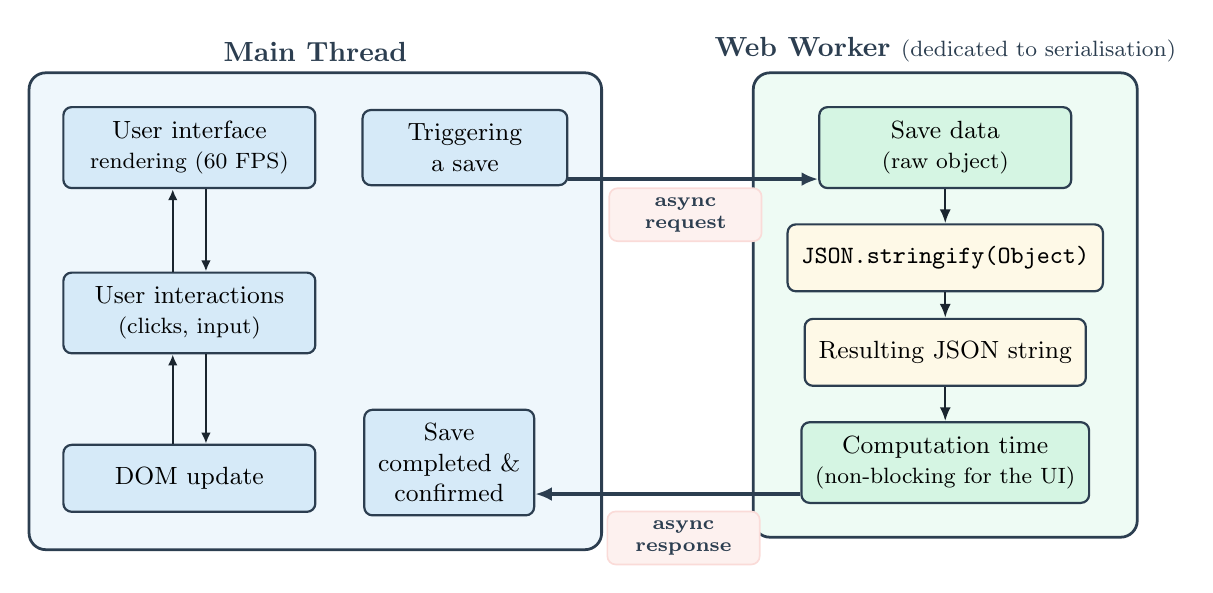
\begin{tikzpicture}[
    every node/.style = {font=\small, align=center},
    % Internal boxes
    box/.style = {
        rectangle, rounded corners=3pt,
        draw=clrBorder, line width=0.8pt,
        minimum width=3.2cm, minimum height=0.85cm,
        inner sep=5pt
    },
    main/.style  = {box, fill=clrInput},
    work/.style  = {box, fill=clrToken},
    proc/.style  = {box, fill=clrProcess},
    % Arrows
    arrow/.style = {-{Latex[length=5pt,width=4pt]},
                    line width=0.8pt, color=clrArrow},
    asyncarrow/.style = {-{Latex[length=6pt,width=5pt]},
                    line width=1.2pt, color=clrBorder},
    lbl/.style   = {font=\scriptsize\itshape, color=clrNote},
    lblbf/.style = {font=\scriptsize\bfseries, color=clrBorder},
    ]

%% ═══════════════════════════════════════════════════════
%% LEFT COLUMN — Main thread
%% ═══════════════════════════════════════════════════════

% Main thread internal nodes (x = -3.8cm)
\node[main] at (-3.8cm,  2.6cm) (ui)
    {User interface\\
     \footnotesize{rendering (60 FPS)}};

\node[main] at (-3.8cm,  0.5cm) (input)
    {User interactions\\
     \footnotesize{(clicks, input)}};

\node[main] at (-3.8cm, -1.6cm) (dom)
    {DOM update};

% Main thread internal arrows (two-way)
\draw[arrow, -{Latex[length=4pt,width=3.5pt]}]
    ([xshift= 6pt]ui.south)    -- ([xshift= 6pt]input.north);
\draw[arrow, -{Latex[length=4pt,width=3.5pt]}]
    ([xshift=-6pt]input.north) -- ([xshift=-6pt]ui.south);

\draw[arrow, -{Latex[length=4pt,width=3.5pt]}]
    ([xshift= 6pt]input.south) -- ([xshift= 6pt]dom.north);
\draw[arrow, -{Latex[length=4pt,width=3.5pt]}]
    ([xshift=-6pt]dom.north)   -- ([xshift=-6pt]input.south);

% Trigger and confirmation boxes
\node[main, minimum width=2.6cm] at (-0.3cm,  2.6cm) (trigger)
    {Triggering\\a save};

\node[main, minimum width=2cm] at (-0.5cm, -1.4cm) (confirm)
    {Save\\completed \& \\ confirmed};

%% ═══════════════════════════════════════════════════════
%% RIGHT COLUMN — Web Worker
%% ═══════════════════════════════════════════════════════

\node[work] at (5.8cm,  2.6cm) (rawdata)
    {Save data\\
     \footnotesize{(raw object)}};

\node[proc] at (5.8cm,  1.2cm) (stringify)
    {\texttt{JSON.stringify(Object)}};

\node[proc] at (5.8cm,  0.0cm) (jsonstr)
    {Resulting JSON string};

\node[work] at (5.8cm, -1.4cm) (calctime)
    {Computation time\\
     \footnotesize{(non-blocking for the UI)}};

% Web Worker internal arrows
\draw[arrow] (rawdata)   -- (stringify);
\draw[arrow] (stringify) -- (jsonstr);
\draw[arrow] (jsonstr)   -- (calctime);

%% ═══════════════════════════════════════════════════════
%% ASYNCHRONOUS ARROWS between zones
%% ═══════════════════════════════════════════════════════

% Request: trigger -> rawdata
\draw[asyncarrow] ([yshift=-0.4cm]trigger.east)
    -- node[lblbf, below=3pt, text width=1.7cm, xshift=-0.1cm, fill=clrOutput!40, line width=0.6pt, draw=clrOutput, rounded corners=3pt] {async request}
    ([yshift=-0.4cm]rawdata.west);

% Response: calctime -> confirm
\draw[asyncarrow] ([yshift=-0.4cm]calctime.west)
    -- node[lblbf, below=6pt, text width=1.7cm, xshift=0.2cm, fill=clrOutput!40, line width=0.6pt, draw=clrOutput, rounded corners=3pt] {async response}
    ([yshift=-0.4cm]confirm.east);

%% ═══════════════════════════════════════════════════════
%% BOUNDING BOXES
%% ═══════════════════════════════════════════════════════

\begin{scope}[on background layer]
  \node[draw=clrBorder, rounded corners=6pt,
        fill=clrInput!40, line width=1pt,
        fit=(ui)(input)(dom)(trigger)(confirm),
        inner sep=12pt,
        label={[font=\normalsize\bfseries, text=clrBorder]
               above:Main Thread}
       ] (mainbox) {};

  \node[draw=clrBorder, rounded corners=6pt,
        fill=clrToken!40, line width=1pt,
        fit=(rawdata)(stringify)(jsonstr)(calctime),
        inner sep=12pt,
        label={[font=\normalsize\bfseries, text=clrBorder]
               above:Web Worker \normalfont\footnotesize (dedicated to serialisation)}
       ] (workerbox) {};
\end{scope}

    \end{tikzpicture}
    \caption{Main thread/Web Worker separation architecture for saving (Author 2026)}
    \label{fig:webworker-architecture}
\end{figure}


Code listing \ref{lst:saveworker} presents the two components of this architecture. On the secondary-thread side, the \texttt{worker} receives, via \texttt{postMessage}, an object containing the current state and the target cookie's name, runs \texttt{JSON.stringify} on its own execution thread, then returns the serialised string together with the cookie name. This coupling guarantees that the \gls{webworker} retains no data between calls: it receives all the information it needs with each message and can be reused for any save operation with no additional initialisation. On the main-thread side, the \gls{webworker} is instantiated only once, when the component is initialised, via \texttt{useEffect}, and is kept in a \texttt{useRef} reference to avoid repeated instantiation. The \texttt{onmessage} callback receives the result asynchronously and triggers the cookie write without ever having blocked the \gls{rendu} thread.

\begin{listing}[H]
\begin{minted}{ts}
// workers/saveWorkers.ts (secondary thread)
self.addEventListener("message",
    (e: MessageEvent<SaveWorkerMessage>) => {
        const { state, cookieName } = e.data;
        const serialized = JSON.stringify(state);
        (self as unknown as Worker).postMessage(
            { serialized, cookieName } satisfies SaveWorkerResponse
        );
    }
);


// VisualNovel/index.tsx (main thread)
const saveWorkerRef = useRef<Worker | null>(null);

useEffect(() => {
    const worker = new Worker(
        new URL('../../../workers/saveWorker.ts', import.meta.url),
        { type: 'module' }
    );
    worker.addEventListener('message',
        (e: MessageEvent<SaveWorkerResponse>) => {
            saveState(e.data.cookieName, e.data.serialized);
        }
    );
    saveWorkerRef.current = worker;
    return () => {
        worker.terminate();
        saveWorkerRef.current = null;
    };
}, []);
\end{minted}
\caption{Implementation of \texttt{saveWorker}: communication protocol between the main thread and the secondary thread (Author 2026)}
\label{lst:saveworker}
\end{listing}

\clearpage


\subsubsubsection{Check}

After several trial runs of the engine, the features implemented during the first iteration were checked and found to be unaffected by the changes made.

To assess the impact of the optimisations on rendering performance, five identical test sessions were recorded using \gls{reactprofiler}, on the version prior to the optimisations (\textit{commit}\footnote{\textbf{Commit}: in \gls{git}, a record of a set of changes made to the source code at a given point in time, identified by a unique fingerprint (hash) allowing it to be reverted to or referenced precisely. \parencite{noauthor_git_nodate}} \texttt{9831b9e}) and on the optimised version. Each session followed the same sequence of interactions on the same test \gls{json} file, in the same browser.

\clearpage

Tables \ref{tab:profiling_before} and \ref{tab:profiling_after} present the four metrics recorded: the total number of \glspl{rendu}, the average duration per \gls{rendu}, the maximum duration observed, and the cumulative duration of all \glspl{rendu} in the session.

\begin{table}[H]
    \centering
    \caption{Performance measurements before optimisation (five sessions)}
    \renewcommand{\arraystretch}{1.5}
    \begin{tabular}{p{0.8cm} p{2.5cm} p{3cm} p{3cm} p{3cm}}
        \hline
        \textbf{No.} & \textbf{Renders} & \textbf{Avg. duration (ms)} & \textbf{Max. duration (ms)} & \textbf{Total duration (ms)} \\
        \hline
        1 & 688 & 0.165 & 2.90 & 113.70 \\
        2 & 689 & 0.166 & 2.90 & 114.50 \\
        3 & 689 & 0.161 & 3.10 & 111.00 \\
        4 & 688 & 0.168 & 3.10 & 115.70 \\
        5 & 688 & 0.163 & 3.00 & 112.10 \\
        \hline
        \textbf{*} & \textbf{688} & \textbf{0.165} & \textbf{3.00} & \textbf{113.70} \\
        \hline
    \end{tabular}
    \par\smallskip{\footnotesize * Median of the five sessions}
    \label{tab:profiling_before}
\end{table}

\begin{table}[H]
    \centering
    \caption{Performance measurements after optimisation (five sessions)}
    \renewcommand{\arraystretch}{1.5}
    \begin{tabular}{p{0.8cm} p{2.5cm} p{3cm} p{3cm} p{3cm}}
        \hline
        \textbf{No.} & \textbf{Renders} & \textbf{Avg. duration (ms)} & \textbf{Max. duration (ms)} & \textbf{Total duration (ms)} \\
        \hline
        1 & 476 & 0.335 & 19.90 & 159.50 \\
        2 & 492 & 0.320 & 18.30 & 157.60 \\
        3 & 492 & 0.327 & 18.40 & 161.10 \\
        4 & 492 & 0.321 & 18.30 & 158.00 \\
        5 & 493 & 0.321 & 18.20 & 158.30 \\
        \hline
        \textbf{*} & \textbf{492} & \textbf{0.321} & \textbf{18.30} & \textbf{158.30} \\
        \hline
    \end{tabular}
    \par\smallskip{\footnotesize * Median of the five sessions}
    \label{tab:profiling_after}
\end{table}

\clearpage

Figures \ref{fig:profiling_renders} and \ref{fig:profiling_maxdur} illustrate, respectively, the change in the number of \glspl{rendu} and in the maximum duration between the two versions.

\begin{figure}[H]
    \centering
    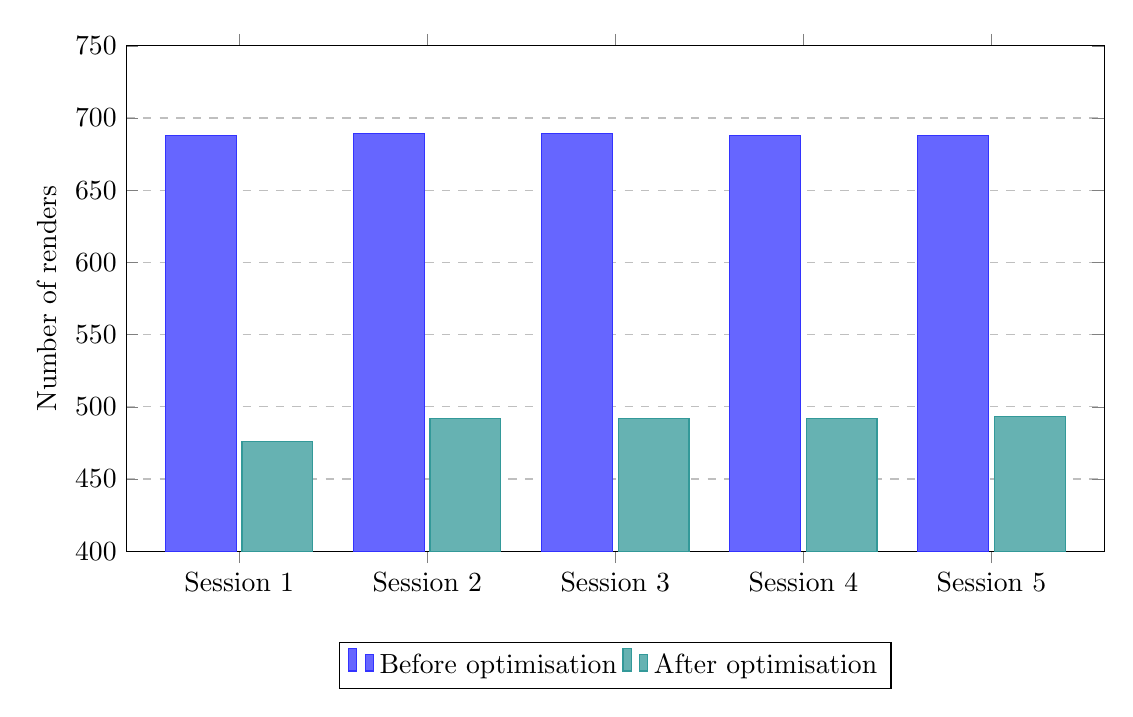
\begin{tikzpicture}
        \begin{axis}[
            ybar,
            bar width=0.9cm,
            width=14cm,
            height=8cm,
            ymin=400,
            ymax=750,
            ylabel={Number of renders},
            xtick=data,
            xticklabels={Session 1, Session 2, Session 3, Session 4, Session 5},
            legend style={at={(0.5,-0.18)}, anchor=north, legend columns=2},
            ymajorgrids=true,
            grid style=dashed,
            enlarge x limits=0.15,
        ]
        \addplot[fill=blue!60, draw=blue!80]
            coordinates {(1,688) (2,689) (3,689) (4,688) (5,688)};
        \addplot[fill=teal!60, draw=teal!80]
            coordinates {(1,476) (2,492) (3,492) (4,492) (5,493)};
        \legend{Before optimisation, After optimisation}
        \end{axis}
    \end{tikzpicture}
    \caption{Number of renders per session before and after optimisation (\textit{commit} \texttt{9831b9e}) measured via React DevTools Profiler (Author 2026)}
    \label{fig:profiling_renders}
\end{figure}

\begin{figure}[H]
    \centering
    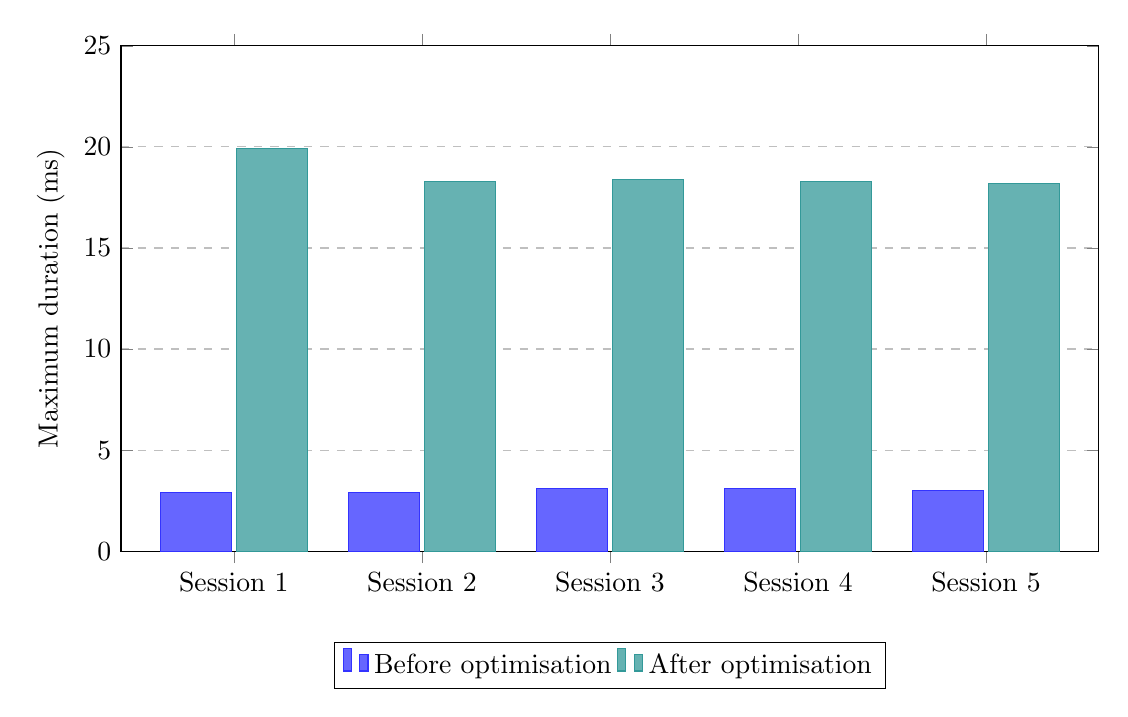
\begin{tikzpicture}
        \begin{axis}[
            ybar,
            bar width=0.9cm,
            width=14cm,
            height=8cm,
            ymin=0,
            ymax=25,
            ylabel={Maximum duration (ms)},
            xtick=data,
            xticklabels={Session 1, Session 2, Session 3, Session 4, Session 5},
            legend style={at={(0.5,-0.18)}, anchor=north, legend columns=2},
            ymajorgrids=true,
            grid style=dashed,
            enlarge x limits=0.15,
        ]
        \addplot[fill=blue!60, draw=blue!80]
            coordinates {(1,2.9) (2,2.9) (3,3.1) (4,3.1) (5,3.0)};
        \addplot[fill=teal!60, draw=teal!80]
            coordinates {(1,19.9) (2,18.3) (3,18.4) (4,18.3) (5,18.2)};
        \legend{Before optimisation, After optimisation}
        \end{axis}
    \end{tikzpicture}
    \caption{Maximum render duration per session before and after optimisation (\textit{commit} \texttt{9831b9e}) measured via React DevTools Profiler (Author 2026)}
    \label{fig:profiling_maxdur}
\end{figure}

\clearpage

The measurements reveal a nuanced result. The number of \glspl{rendu} decreased by 28.5\% (688 → 492), confirming the effect of \texttt{React.memo}: unnecessary \glslink{rendu}{re-renders} were eliminated. On the other hand, the average duration per \gls{rendu} increased (0.165ms → 0.321ms), and the peak maximum rose from 3ms to 18.3ms. This behaviour is consistent with the precomputation strategy adopted by the \texttt{Typewriter} component: the computational cost is concentrated on the initial \gls{rendu} rather than spread across each displayed character. For comparable overall performance, the optimised version therefore places a lighter load on the browser's main thread over the course of a session.


\subsubsubsection{Act}

With the optimisations made during this iteration having met their main objective, the next area of work had already been identified since the first iteration: error handling and data validation. With the engine now performant, it was time to ensure it was also robust when faced with invalid or incomplete \gls{json} files. The third iteration was therefore dedicated to researching and implementing a \gls{schema} validation system.


\subsubsection{Third Iteration: Security and Robustness}

\subsubsubsection{Plan}

The objective of this iteration was to address the main limitation identified during the previous iterations: the absence of formal validation of the \acrshort{json} files supplied by the author. Without a verification mechanism, a syntactically invalid file, or one that did not conform to the expected \gls{schema}, could put the engine into an indeterminate state, with no actionable feedback for the author. Integrating the \gls{zod} \gls{librairie}, presented in Section \ref{sec:zod}, was the response to this gap.

Discovering \gls{zod} was not the result of a targeted search, but of a chance encounter on GitHub, where the \gls{librairie} appeared frequently in \gls{ts} projects dealing with \gls{schema} validation. Before adopting it, two alternatives were evaluated: TypeBox\footnote{\textbf{TypeBox}: \gls{json}-based \gls{ts} \gls{schema} validation \gls{librairie}, developed by Haydn Paterson \parencite{noauthor_typebox_nodate}} and ArkType\footnote{\textbf{ArkType}: validation and type-inference \gls{librairie} for \gls{ts}, focused on performance and a \gls{syntaxe} inspired by the language's native notation \parencite{noauthor_arktype_nodate}}. TypeBox offers an approach similar to \gls{zod}, while ArkType relies on a noticeably different \gls{syntaxe}, which proved less immediate to pick up. The choice ultimately fell on \gls{zod} for the conciseness and readability of its \gls{syntaxe}, an important criterion when it comes to keeping the code accessible to the project's potential contributors.

\clearpage

This iteration also made it possible to implement several \textit{Can} features identified in Table \ref{tab:objectifs_moscow}, which available time had not allowed integrating during the previous iterations: displaying character \glsplit{sprite} with dynamic positioning, transitions between scenes and dialogues, font management via \acrshort{css} variables, and support for a dynamic \glsit{placeholder} for input fields.


\subsubsubsection{Do}

The integration of \gls{zod} was built around two distinct validation \glspl{schema}. The first, \texttt{storySchema}, describes the expected structure of the scenario's \acrshort{json} file: node types, presence of required fields, allowed values for enumerated properties. The second, \texttt{saveSchema}, covers the structure of save files, in order to detect and reject any corrupted or manually modified file before it is passed to the engine. In case of a discrepancy from the defined \gls{schema} (missing field, incorrect type, invalid structure), \gls{zod} returns an explicit error message precisely indicating the location and nature of the problem, which constitutes a deterministic error-detection mechanism and direct feedback for the author.

Code listing \ref{lst:storyschema} presents an excerpt of \texttt{VNStorySchema}. Validation operates on two levels. The first is declarative: each field of the \gls{json} file is explicitly typed via \gls{zod} primitives (\texttt{z.string()}, \texttt{z.number().positive()}, \texttt{z.enum([...])}), which makes it possible to catch at runtime any missing field, incorrect type, or value outside the allowed options. The second level, implemented via \texttt{superRefine}, performs cross-field semantic validation that cannot be expressed with types alone: it checks that the scene referenced by \texttt{startingScene} does exist in the \texttt{story} block, and that every navigation target (the \texttt{next} fields of dialogues and options) points to a declared scene. In case of a discrepancy, \texttt{ctx.addIssue} produces an error message including the exact path of the offending field, as illustrated in Figure \ref{fig:zod_erreurs}.

\begin{listing}[H]
\begin{minted}{ts}
const DialogueSchema = z.object({
    next: z.string().optional(),
    options: z.array(OptionSchema).optional(),
});

export const VNStorySchema = z.object({
    settings: SettingsSchema,
    story: z.record(z.string(), SceneTypeSchema),
}).superRefine((data, ctx) => {
    if (!data.story[data.settings.startingScene]) {
        ctx.addIssue({
            code: "custom",
            message: `"${data.settings.startingScene}" does not exist in Story`,
            path: ["settings", "startingScene"],
        });
    }
    for (const [sceneId, scene] of Object.entries(data.story)) {
        scene.dialogues.forEach((dialogue, i) => {
            const refs = [
                ...(dialogue.next ? [{val: dialogue.next, path: ["next"]}] : []),
                ...(dialogue.options ?? []).map(o => ({val: o.next, path: ["options"]})),
            ];
            refs.forEach(({val, path}) => {
                const target = val.split(":")[0];
                if (!data.story[target] && target !== END_STORY_TOKEN) {
                    ctx.addIssue({
                        code: "custom",
                        message: `Scene "${target}" does not exist`,
                        path: ["story", sceneId, "dialogues", i, ...path],
                    });
                }
            });
        });
    }
});
\end{minted}
\caption{Excerpt of \texttt{VNStorySchema}: declarative validation and semantic verification of navigation references (Author 2026)}
\label{lst:storyschema}
\end{listing}

\clearpage

To cover error cases systematically, dedicated test files were added to the repository in a \texttt{tests/} folder. These files intentionally represent invalid scenarios: \acrshort{json} with broken \gls{syntaxe} (missing comma, unclosed quotation mark), files with missing required fields, and files with incorrect-type values. These files are excluded from the production \glsit{build} via a dedicated \gls{vite} \glsit{plugin}.


\subsubsubsection{Check}

The \glslink{negativetesting}{negative tests} carried out at the end of this iteration covered all of the cases described above. In each case, \gls{zod} returned an explicit error message and the engine remained in a stable state, confirming the expected behaviour, as illustrated in Figure \ref{fig:zod_erreurs}.

\begin{figure}[H]
    \centering
    \begin{subfigure}[b]{0.47\textwidth}
        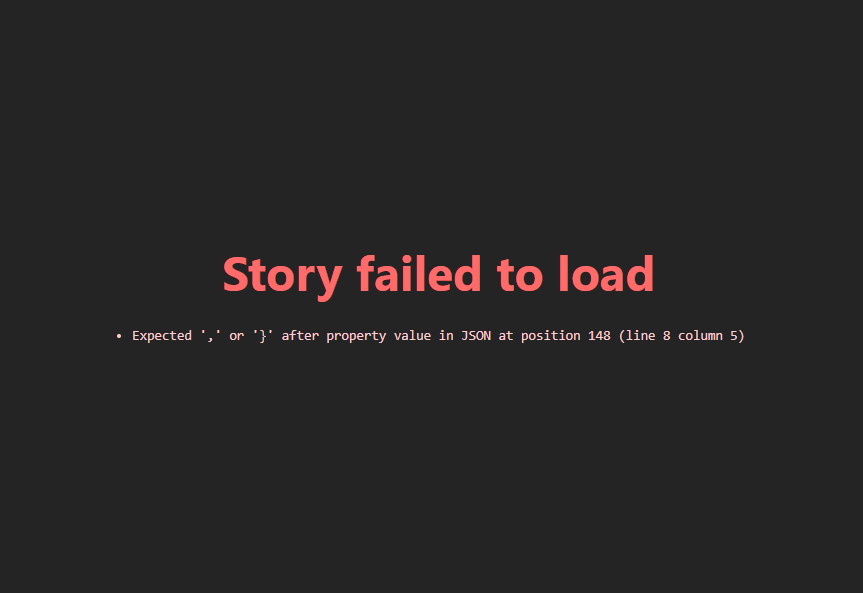
\includegraphics[height=4.85cm]{img/zod_invalid_syntax_1.png}
        \caption{JSON syntax error}
    \end{subfigure}
    \hfill
    \begin{subfigure}[b]{0.47\textwidth}
        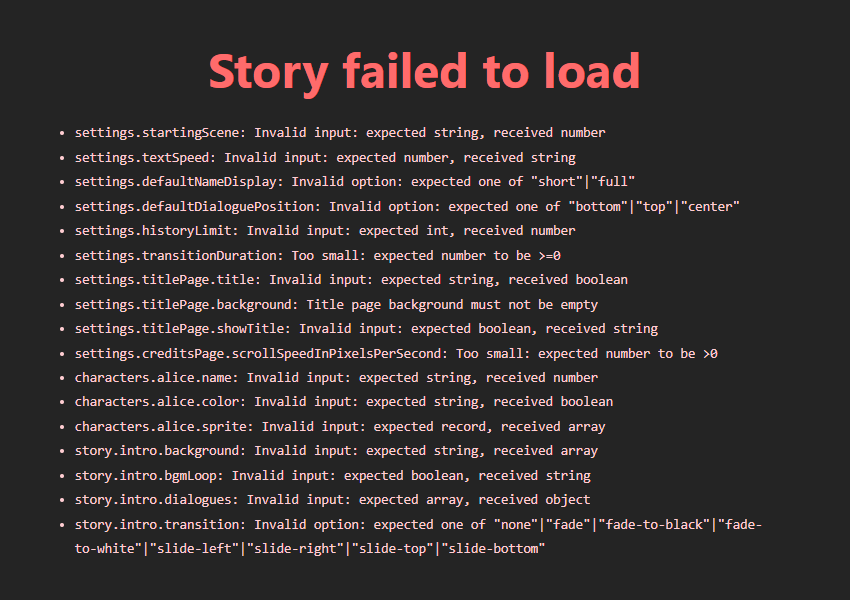
\includegraphics[height=4.85cm]{img/zod_missing_field_1.png}
        \caption{Missing required fields}
    \end{subfigure}
    \caption{Error messages returned by Zod when validating the JSON file (Author 2026)}
    \label{fig:zod_erreurs}
\end{figure}

Save file validation was also tested by supplying manually modified files, which were correctly rejected with an error message surfacing all the way up to the title screen.

\clearpage

Figure \ref{fig:NamelessStoryFinal} presents the state of the engine at the end of these three iterations. The remark made in footnote \ref{fn:zoom175} about browser zoom also applies to these screenshots. The \gls{json} file used for this screenshot differs from the one used in the first iteration: rather than a short story, it is a demo (\textit{"The Feature Tour"}) running through all the features implemented in the engine.

\begin{figure}[H]
    \centering
    \begin{subfigure}[b]{0.47\textwidth}
        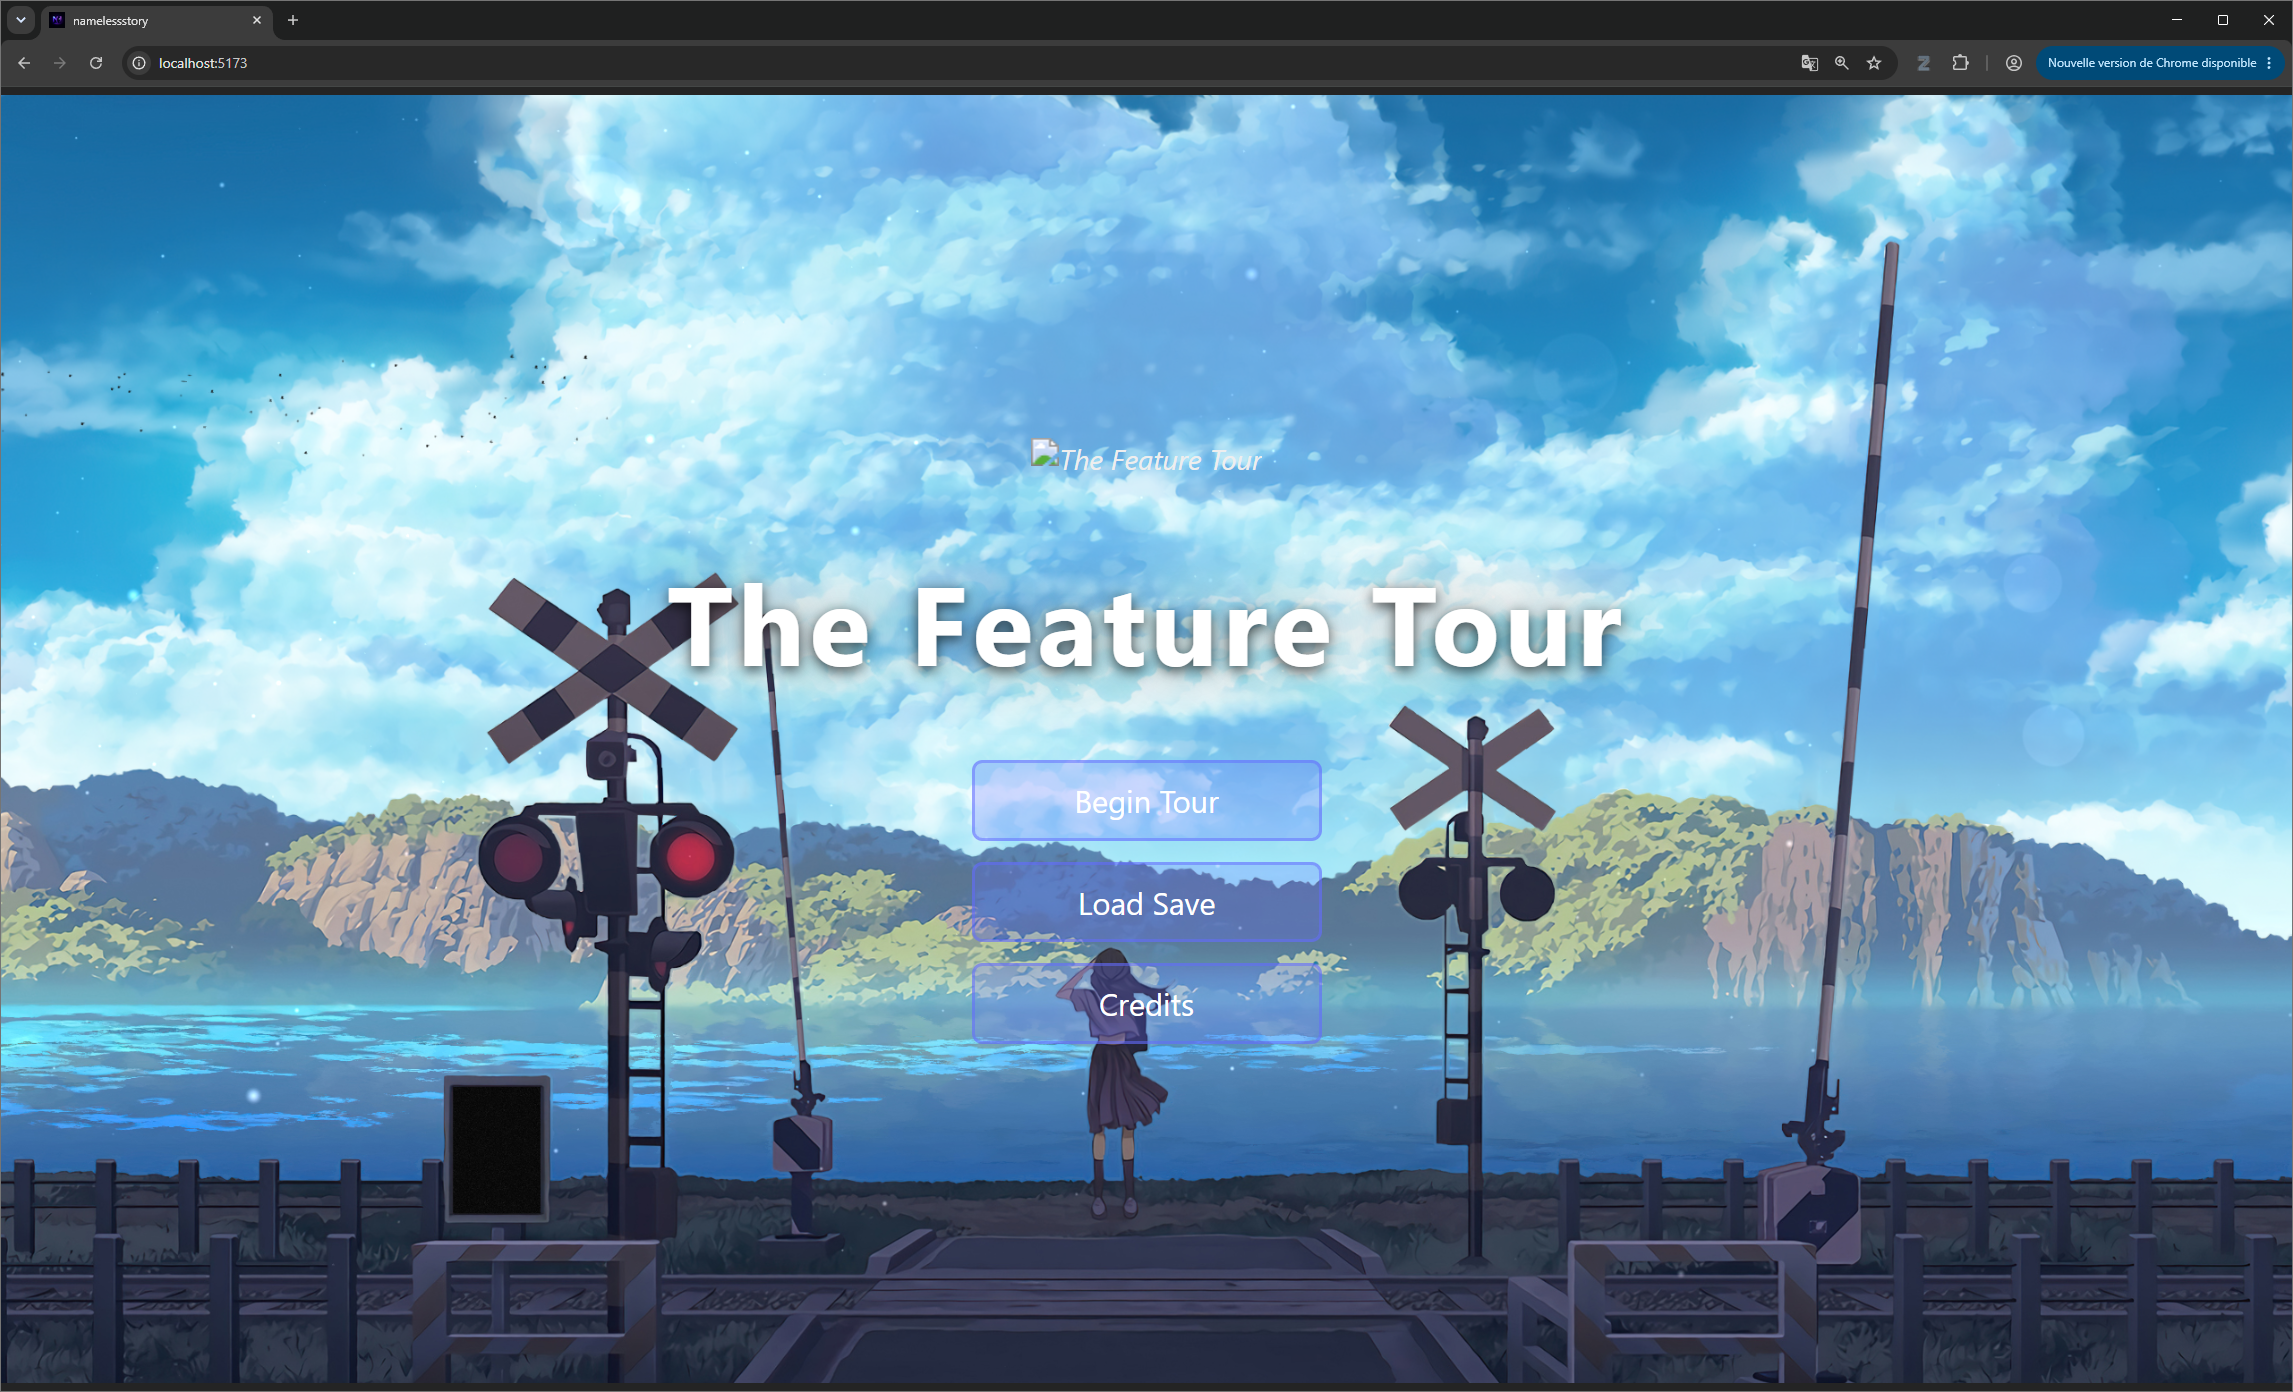
\includegraphics[width=\textwidth]{img/NamelessStory_final_home.png}
        \caption{Title screen}
    \end{subfigure}
    \hfill
    \begin{subfigure}[b]{0.47\textwidth}
        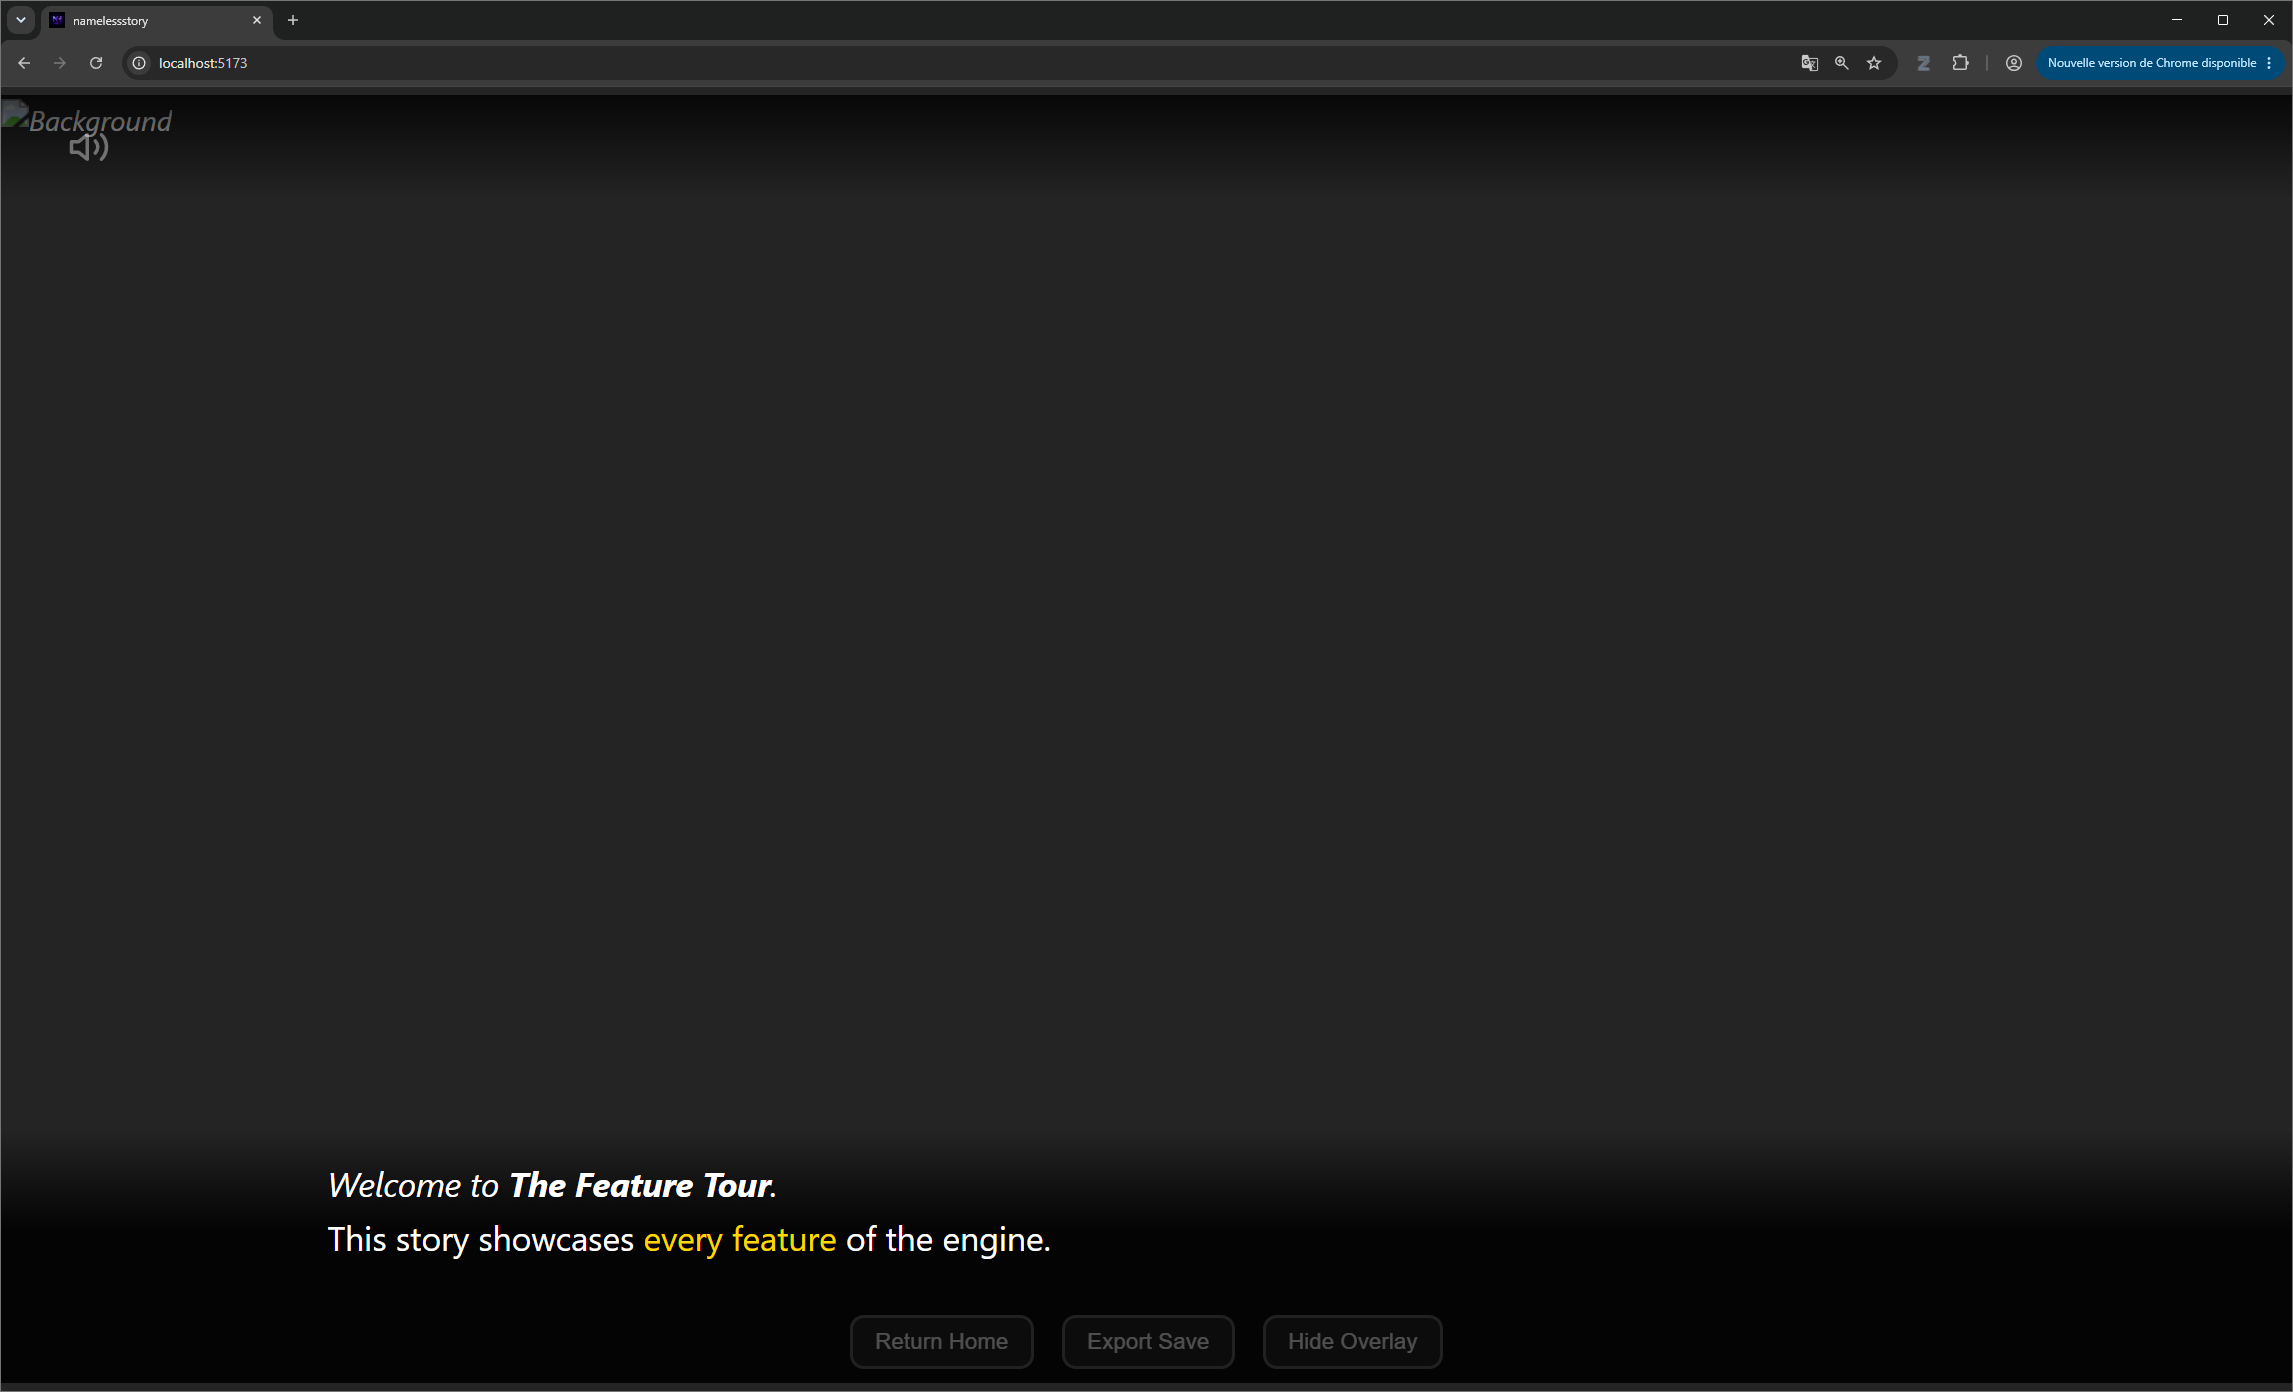
\includegraphics[width=\textwidth]{img/NamelessStory_final_text.png}
        \caption{Dialogue display}
    \end{subfigure}
    \caption{\nsits at the end of the third iteration (Author 2026)}
    \label{fig:NamelessStoryFinal}
\end{figure}


\subsubsubsection{Act}

At the end of this iteration, all of the \textit{Must} and \textit{Should} objectives defined in Table \ref{tab:objectifs_moscow} had been met. Several \textit{Can} features were also integrated. The remaining out-of-scope features (notably a built-in scenario editor and advanced handling of complex narrative branching) are identified as future development directions in Chapter \ref{chap:resultats}.


\section{Results}
\label{chap:resultats}

\subsection{Summary of Results}

This chapter brings together the results obtained over the three development iterations of \nsit. I present both the quantitative measurements and the more qualitative observations that allowed me to evaluate the work carried out: achievement of the functional objectives, performance observed, and robustness brought by \gls{json} file validation.



\subsubsection{Achievement of Objectives (MoSCoW)}

Table \ref{tab:resultats_moscow} summarises the progress status of the objectives defined for the project. It provides a quick view of what was achieved, partially achieved, or left for a future version.

\begin{table}[H]
    \centering
    \caption{Completion of the MoSCoW objectives}
    \renewcommand{\arraystretch}{1.4}
    \begin{tabular}{p{1.6cm} p{5.5cm} p{6cm}}
        \hline
        \textbf{Priority} & \textbf{Feature} & \textbf{Status and remarks} \\
        \hline
        Must & "Typewriter" effect (\texttt{Typewriter} component) & Achieved. Behaviour optimised through precomputation of \glslink{snaphtml}{HTML snapshots} and delay calculation (see Section \ref{sec:optim_react} and Listing \ref{lst:typewriter}). \\
        \addlinespace
        Must & Navigation between scenes & Achieved. The "Scene" and "Dialogue" components handle progression and the \texttt{next} key for navigation. \\
        \addlinespace
        Must & Handling of choices and branching & Achieved. Selectable options leading to targeted scenes or dialogues. \\
        \addlinespace
        Should & Input handling (fields) & Achieved. Support for a dynamic \glsit{placeholder} and basic handling of user input. \\
        \addlinespace
        Can & Additional features (\glsplit{sprite}, transitions, fonts) & Partially achieved: \glsplit{sprite} and transitions implemented; advanced save handling and a built-in editor not delivered (future directions). \\
        \hline
    \end{tabular}
    \label{tab:resultats_moscow}
\end{table}



\subsubsection{Performance Metrics}

To measure the effect of the optimisation iteration, I used \gls{reactprofiler} on five identical sessions, before and after the optimisations. The relevant measurements are set out in Table \ref{tab:metriques_performance}, based on the median of five sessions.

\begin{table}[H]
    \centering
    \caption{Performance metrics before/after optimisation (medians over five sessions)}
    \renewcommand{\arraystretch}{1.4}
    \begin{tabular}{p{6cm} p{3cm} p{3cm}}
        \hline
        \textbf{Metric} & \textbf{Before} & \textbf{After} \\
        \hline
        Number of \glspl{rendu} & 688 & 492 \\
        \addlinespace
        Average duration per \gls{rendu} & 0.165 ms & 0.321 ms \\
        \addlinespace
        Maximum duration observed & 3.0 ms & 18.3 ms \\
        \addlinespace
        Cumulative session duration & 113.7 ms & 158.3 ms \\
        \hline
    \end{tabular}
    \label{tab:metriques_performance}
\end{table}

These results (Tables \ref{tab:profiling_before}, \ref{tab:profiling_after} and \ref{tab:metriques_performance}, Figures \ref{fig:profiling_renders} and \ref{fig:profiling_maxdur}) show a clear trade-off. The use of \gls{memoisation} and precomputation mechanisms markedly reduces the number of unnecessary \glslink{rendu}{re-renders}, a 28.5\% reduction, but also concentrates part of the computational cost at the initial preparation stage. In practice, this makes the experience smoother during the session, at the cost of a somewhat higher cost on certain isolated \glspl{rendu}. For this project, this trade-off seems consistent with the main objective: avoiding repeated blocking of the main thread.



\subsubsection{Robustness and Validation}

Integrating the \gls{zod} \gls{librairie} made it possible to introduce declarative and semantic validation of \gls{json} files (\texttt{storySchema} and \texttt{saveSchema} \glspl{schema}). The \glslink{negativetesting}{negative tests} added confirm that:

\begin{itemize}
    \item \gls{json} \gls{syntaxe} errors and missing required fields are detected and surfaced via explicit messages, see Figure \ref{fig:zod_erreurs}.
    \item Corrupted save files are rejected before being injected into the application.
\end{itemize}

These results partially answer the research question: the declarative format (\gls{json} + \gls{schema}) makes the engine deterministic and verifiable, but without a suitable editing tool the non-developer author remains exposed to the \gls{syntaxe} constraint.



\subsection{Evaluation and Self-Reflection}

\subsubsection{Media Project Evaluation}

On the technical side, the main gains were portability, robustness, and the performance improvements observed thanks to \gls{memoisation} and precomputation. The profiling measurements showed a notable reduction in the number of \glspl{rendu}, at the cost of a higher one-off cost for certain initial \glspl{rendu}. This trade-off remains consistent with the goal of avoiding continuous blocking of the main thread.

The limitations identified concern accessibility for non-developer authors, the still-limited readability of the \gls{json} format, and the absence of a guided editor. In addition, some advanced features, such as complex conditional branching, a built-in editor, or advanced save handling, remain out of scope for this version and represent future development directions.

In response to the research question, the architecture based on a declarative format shows that it is technically possible to allow the creation of interactive content without a \glsit{backend}, with automatic validation to prevent runtime errors. However, for non-developer authors to genuinely be able to create content without technical help, an additional tooling layer still needs to be added, for example a guided editor or a conversion from a more readable format.



\subsubsection{Personal Reflection}

I carried out the entire project alone: design, development, testing, and writing. The \glsit{pdca} method helped me prioritise the essential features, but I also had to deal with personal and professional constraints, notably health and workload, which slowed down certain stages.

Integrating \gls{zod} is an achievement I am proud of: providing clear error messages markedly improved robustness. Likewise, building the project in \gls{ts} helped prevent errors and made the code more maintainable. I also gained new skills in \gls{reactjs} optimisation (\texttt{useMemo}, \texttt{React.memo}) and in using \gls{webworker} to offload certain processing.

The choice of script format (\gls{json}) proved constraining from the author's point of view: although pragmatic for development, it remains less suited to non-technical writers. Due to lack of time, I gave up on implementing rich conditional branching, which would have increased the implementation's complexity.

\clearpage

As noted in Chapter \ref{chap:methodologie}, I was not able to confront this work with professional opinion. My attempts to contact \gls{vn} developers and web developers, carried out since January 2026, went unanswered. The evaluation presented here therefore relies on the \glsit{poc} built and on my own analysis, without specialised external validation, which is a limitation to keep in mind when reading the results above.

If I had to start over, I would integrate a schema validator (\gls{zod} or equivalent) earlier, and I would spend more time designing a guided editing tool. The immediate next steps for the project are to:

\begin{itemize}
    \item build a prototype guided editor with real-time validation;
    \item conduct user testing (5–8 participants) to measure the format's accessibility;
    \item progressively improve narrative branching and the technical documentation.
\end{itemize}

% End of Results chapter


\section{Conclusion}
\label{chap:conclusion}

\subsection{Synthèse}
Ce mémoire a présenté la conception, l’implémentation et l’évaluation de \nsit, un moteur de \acrlong{vn} web fondé sur un format de script déclaratif en \gls{json}. L’idée de départ était simple: vérifier si une architecture de ce type pouvait réellement permettre à des auteurs non-développeurs de créer et de publier des récits interactifs sans passer par une installation locale ou une phase de compilation.

Au fil du travail, j’ai défini un \gls{schema} de script, construit un \glsit{runtime} web en \gls{ts}/\gls{reactjs}, optimisé les composants les plus coûteux, notamment \texttt{Typewriter}, puis ajouté une validation d’exécution via \gls{zod}. Trois itérations successives, centrées sur les bases, l’optimisation et la robustesse, ont permis d’atteindre les objectifs classés \textit{Must} et \textit{Should}: affichage progressif du texte, navigation entre scènes, gestion des choix, validation du format et gestion basique des saisies. Certaines fonctions \textit{Can}, comme les \glsplit{sprite}, les transitions ou la sauvegarde déléguée à un \gls{webworker}, ont également été amorcées.


\subsection{Réponse à la problématique et bilan critique}
La question de recherche portait sur la capacité d’une architecture de moteur de \gls{vn} web, fondée sur un format déclaratif, à permettre à des auteurs non-développeurs de créer du contenu interactif. Sur le plan technique, la réponse est positive: j’ai montré qu’il était possible de décrire un récit interactif dans un fichier déclaratif et de l’exécuter directement dans un navigateur, avec des mécanismes de validation et des messages d’erreur exploitables.

En revanche, l’évaluation met aussi en évidence une limite plus nette du point de vue de l’auteur. Le format \gls{json}, même s’il est adapté au moteur, reste sensible aux erreurs de syntaxe et peu confortable pour une personne qui ne vient pas du développement. Sans éditeur guidé, validation en temps réel ou modèles prêts à l’emploi, l’approche déclarative seule ne suffit pas à rendre la création totalement autonome. Par ailleurs, certains choix techniques, comme la précomputation des \glslink{snaphtml}{snapshots} ou la délégation de traitements à un \gls{webworker}, améliorent le comportement du moteur, mais introduisent aussi des compromis qu’il faut accepter selon le contexte d’usage.

En résumé, l’architecture est viable et propre sur le plan technique, mais elle doit encore être entourée d’outils pensés pour l’écriture afin de répondre pleinement à l’objectif initial.


\subsection{Pistes de développement}

\subsubsection{Pistes de développement du Media Project}
Pour rendre la solution réellement utilisable par des auteurs non-développeurs, plusieurs évolutions me paraissent prioritaires :

\begin{itemize}
    \item Développer un éditeur guidé avec validation en temps réel (prévisualisation, messages d'erreur explicites, modèles), afin de masquer la complexité syntaxique du \gls{json}.
    \item Ajouter des outils de conversion et d'import (par ex. importer depuis un format plus lisible ou depuis un langage narratif type Ink) pour réduire la courbe d'apprentissage.
    \item Étendre le moteur avec des embranchements conditionnels, des variables de scénario plus riches et une API d'extensions pour permettre des fonctionnalités avancées sans modifier le cœur du \glsit{runtime}.
    \item Automatiser la chaîne de publication (intégration continue → déploiement statique) et fournir des \textit{workflows} \textit{one-click}\footnote{\textbf{Workflow} « one-click »: enchaînement automatisé d'étapes techniques (ici, de compilation et de déploiement) déclenché par une seule action de l'utilisateur.} pour la mise en ligne des histoires.
    \item Améliorer l'accessibilité et la documentation utilisateur (guides pas-à-pas, exemples, galerie de templates).
\end{itemize}

\clearpage


\subsubsection{Pistes de recherche}
Plusieurs axes de recherche découlent de ce travail :

\begin{itemize}
    \item L'ajout d'un éditeur graphique ou assisté, visuel ou nodal, superposé au format déclaratif, qui masquerait la syntaxe \gls{json} tout en conservant les avantages du texte brut, comme le suivi de version ou la portabilité.
    \item La conception d'un langage narratif intermédiaire, plus proche du langage naturel, qui serait ensuite compilé vers le \gls{schema} \gls{json} du moteur, à la manière de langages dédiés comme Ink ou Twine.
    \item L'intégration d'assistants d'écriture fondés sur des modèles de langage, capables de générer ou de restructurer des fragments narratifs directement dans le format déclaratif.
    \item L'extension du modèle déclaratif vers une logique narrative plus riche, avec des variables d'état persistantes ou des embranchements conditionnels, et son effet sur la lisibilité du format pour un auteur non-développeur.
    \item La standardisation ou l'interopérabilité d'un format déclaratif de \gls{vn}, de façon à ce qu'un même script puisse être exécuté par plusieurs moteurs ou plateformes.
    \item La prise en compte de l'accessibilité, notamment pour les lecteurs d'écran et l'internationalisation, directement au niveau du schéma déclaratif plutôt que comme une couche ajoutée après coup.
\end{itemize}

Ces pistes ouvrent des perspectives complémentaires à ce travail, en interrogeant la manière dont le format déclaratif pourrait évoluer pour concilier simplicité d'accès et richesse narrative.



% ==========================
% ==========================
% ==========================



\clearpage

\include{chapters/bibliographie}

\end{document}